\chapter{Wind-stress with positive surface buoyancy forcing
   (WSwPSBF)}
\label{chapter:WSwPSBF}

In this chapter, we document tests configured with a constant zonal
wind stress and a non-negative surface buoyancy forcing realized by a
heat flux.  These tests only exercise the local downgradient diffusive
portion of KPP.  Although relatively simple, the tests have proven
useful for ensuring that implementation details are consistent across
ocean models making use of CVMix/KPP.  They furthermore illustrate a
nontrivial dependence of the boundary layer depth on vertical
resolution.

\minitoc

\section{Physics of the experiments}

In these test cases, buoyancy is forced at the surface via a surface
heat flux.  To help develop notation, we express the finite-volume
heat equation acting on the top grid cell as
\begin{equation}
  \mbox{C}_{\mbox{\footnotesize p}} \left(   \frac{\partial  \, (\Theta \, \rho \, \mathrm{d}z )}{\partial t}  \right) =  
  Q + F_{\mbox{\footnotesize diffusive}} + F_{\mbox{\footnotesize non-local}}.
\label{eq:surface-heat-equation}
\end{equation}
The following terms appear in this equation.
\begin{itemize}
\item The grid cell thickness, $\mathrm{d}z$, is generally a function
  of time, as in MPAS-ocean and MOM6, in which case we keep it inside
  the time derivative to ensure a flux-form budget.  If the cell
  thickness is static, as in POP, then it can be removed from the time
  derivative.

\item The {\it in situ} density factor, $\rho$, is replaced by the
  constant reference density $\rho_{0}$ when making the Boussinesq
  approximation.

\item The surface boundary heat flux, $Q$, crosses the top of the
  surface cell.  It is specified in these tests according to the
  details in Table \ref{table:kpp-model-configuration} discussed in
  Section \ref{section:configuration-details-WSwPSBF}.

\item The diffusive heat flux, $F_{\mbox{\footnotesize diffusive}}$,
  arises from the local downgradient diffusive portion of the KPP
  scheme.  This flux passes through the bottom face of the top grid
  cell.

\item The non-local KPP term, $F_{\mbox{\footnotesize non-local}}$,
  vanishes in these tests since we are only considering positive
  buoyancy forcing.

\end{itemize}


\section{Configuration details}
\label{section:configuration-details-WSwPSBF}

We here provide configuration details.  Note that each ocean model
makes the Boussinesq approximation for these tests.


\subsection{Vertical grids and time steps}

We consider four vertical grid configurations for each ocean model
(MOM6, MPAS-ocean, and POP).  Three tests are identical across the
models, based on uniform vertical grids of $\Delta z = 20~\mbox{cm}$,
$\Delta z = 1~\mbox{m}$ and $\Delta z = 10~\mbox{m}$.  These tests
serve as a platform to examine differences arising from coarsening the
vertical resolution.  The final test is based on a global
configuration that uses non-uniform grid spacing.  This test uses
grids unique to each ocean model, based on respective global model
configurations.

%%%%%%%%%%%%%%%%%%%% model configurations%%%%%%%%%%%%%%%%%%%%%%%%
\begin{table}[h!t]
\centering{
\begin{tabular}{|c|c|c|c|}
\hline 
{\sc model}                        & {\sc vertical grid spacing/grid points}    & {\sc bottom depth}   &    {\sc time step (secs)} \\
\hline uniform-20cm           & $\Delta z = 20~\mbox{cm}$                     & $400~\mbox{m}$      & $\Delta t = 20 * 60$     \\                               
\hline uniform-1m                 & $\Delta z = 1~\mbox{m}$                      & $400~\mbox{m}$      & $\Delta t = 20 * 60$     \\                               
\hline uniform-10m               & $\Delta z = 10~\mbox{m}$                    & $400~\mbox{m}$      & $\Delta t = 20 * 60$      \\                               
\hline MOM6-CM4             &  75                                                           & $6500~\mbox{m}$    & $\Delta t = 20 * 60$      \\
\hline MPAS-ACME             &  ??                                                             & ??                            & $\Delta t = ??$             \\
\hline POP-CESM                & ??                                                            & ??                              & $\Delta t = ??$             \\
\hline
\end{tabular}
}
\caption{Model vertical grid spacing, bottom depth,  and time steps for the CVMix column tests.}
\label{table:kpp-model-configuration}
\end{table}
%%%%%%%%%%%%%%%%%%%%%%%%%%%%%%%%%%%%%%%%%%%%%%%%%%%%%%%%%%%%%%%%%%%%%%%%


\subsection{Basic constants and linear equation of state}

The basic constants used for the tests are given by the gravitational
acceleration, the Coriolis parameter, and the heat capacity, each of
which are global constants.
\begin{subequations}
\begin{align}
 g &= 9.80616~\mbox{m}~\mbox{s}^{-2}
 \\
 f &= 1.0 \times 10^{-4}~\mbox{s}^{-1}
 \\
\mbox{C}_{\mbox{\footnotesize p}} &= 3992.1~\mbox{J}~\mbox{kg}^{-1}~\mbox{K}^{-1}. 
\end{align}
\end{subequations}
We offer the following comments.
\begin{itemize}
\item A non-zero Coriolis parameter allows for inertial oscillations
  in the vertical column test cases, with periods 
\begin{equation}
   T_{\mbox{\footnotesize inertial}} = \frac{2 \, \pi}{f} = 0.73~\mbox{day}.
\label{eq:inertial-period}
\end{equation}
Consequently, inertial oscillations are a prominent feature in the
velocity field realized in these tests.

\item The heat capacity is needed to convert from a heat flux to a
  temperature flux.  The chosen value accords with the first five
  significant digits of the \cite{TEOS2010} value.

\end{itemize}
The equation of state for density is linear, and a function only of
temperature and salinity 
\begin{equation}
\rho = \rho_0 - \alpha \, (\Theta - \Theta_0) + \beta \, (S-S_0).
\label{eq:linear-eos}
\end{equation}
The equation of state constants are given by 
\begin{subequations}
\begin{align}
 \rho_0 &= 1025.022~\mbox{kg}~\mbox{m}^{-3}
\label{eq:linear-eos-paramA}
 \\
\alpha &= 2.55 \times 10^{-1}~\mbox{kg}~\mbox{m}^{-3}~^{\circ}C^{-1}
\\
\beta &= 7.64\times10^{-1}~\mbox{kg}~\mbox{m}^{-3}~\mbox{ppt}^{-1}
 \\
T_0  &=  19^{\circ}C 
\\
S_0 &=  35~\mbox{ppt}.
\label{eq:linear-eos-paramB}
\end{align}
\end{subequations}


\subsection{Initial Conditions}

We start the velocity field with zero value throughout the column
\begin{equation}
 {\bf v} = 0.
\end{equation}
Surface stress imparts a vertical shear in the horizontal velocity.  A
vertical viscosity will then transfer momentum vertically.  Salinity
is initialized to the constant value
\begin{equation}
 S = S_{0}.
\end{equation}
There are no salt fluxes through the boundaries, so that salinity
remains constant throughout these tests.  The temperature is
initialized with a linear vertical stratification
\begin{subequations}
\begin{align}
 \Theta(z) &= \Theta_s + \Gamma \, z  
\\
 \Theta_s &= 15.0^{\circ}C 
\label{eq:thetas}
\\
 \Gamma  &= 0.01^{\circ}C~\mbox{m}^{-1}. 
\end{align}
\end{subequations}
Even without a surface buoyancy flux, temperature will evolve in the
presence of a nonzero vertical diffusivity.  With the linear equation
of state (\ref{eq:linear-eos}) and parameters
(\ref{eq:linear-eos-paramA})-(\ref{eq:linear-eos-paramB}), the initial
vertical temperature stratification leads to an initial buoyancy
frequency
\begin{subequations}
\begin{align}
 N &= \left(-\frac{g}{\rho_{0}} \frac{\partial \rho}{\partial z} \right)^{1/2}
 \\
   &= \left( \frac{g \, \alpha \, \Gamma}{\rho_{0}} \right)^{1/2}
\\
  &= 4.94 \, \times \, 10^{-3}~\mbox{s}^{-1}
 \\
 &= 49.4 \, f.
\end{align}
\end{subequations}


\subsection{Boundary conditions}

We assume the following boundary conditions.
\begin{itemize}

\item Zero buoyancy flux passes through the ocean bottom.

\item We assume a constant zonal stress and zero meridional stress at
  the ocean surface
\begin{subequations}
\begin{align}
 \tau^{x} &=  0.1~\mbox{N}~\mbox{m}^{-2}
 \\
 \tau^{y} &=  0.
\end{align} 
\end{subequations}

\item Specification of the surface heat flux, $Q$ (see equation
  (\ref{eq:surface-heat-equation})), distinguishes the following three
  experiments (see Table \ref{table:kpp-test-case-WSwPSBF}).

\begin{itemize} 

\item {\sc WSwPSBF.A} uses zero surface heat flux, $Q=0$.

\item {\sc WSwPSBF.B} uses a constant surface heat flux,
  $Q=100~\mbox{W}~\mbox{m}^{-2}$.

\item {\sc WSwPSBF.C} uses a restoring surface boundary condition
  given by
\begin{equation}
 Q =  \rho_o \, \mbox{C}_{\mbox{\footnotesize p}} \, w_{\mbox{\footnotesize piston}} \, (\Theta - \Theta_{\mbox{\footnotesize restore}} ),
\label{eq:heat-flux-restoring}
\end{equation}
 where the restoring temperature is 
\begin{equation}
\Theta_{\mbox{\footnotesize restore}}  = \Theta_s + 10^{\circ}C,
\label{eq:restoring-temp}
\end{equation}
 and the piston velocity is 
\begin{equation}
  w_{\mbox{\footnotesize piston}} = 0.5~\mbox{m}~\mbox{day}^{-1}. 
\end{equation}
With these parameters, the restoring boundary condition produces a
heat flux, per degree temperature deviation $\Theta -
\Theta_{\mbox{\footnotesize restore}}$, given by
\begin{subequations}
\begin{align}
 \frac{Q}{(\Theta - \Theta_{\mbox{\footnotesize restore}} )} &= \rho_o \, \mbox{C}_{\mbox{\footnotesize p}} \, w_{\mbox{\footnotesize piston}}
 \\
 &= 23.68~\mbox{W}~\mbox{m}^{-2}~\mbox{K}^{-1}.  
\end{align}
\end{subequations}
That is, with $\Theta - \Theta_{\mbox{\footnotesize restore}} =
1~\mbox{K}$, we have $Q = 23.68~\mbox{W}~\mbox{m}^{-2}$.  This heat
flux will always be non-negative, causing the ocean temperature to
initially increase quite rapidly as driven by
$\Theta_{\mbox{\footnotesize restore}} - \Theta_s = 10^{\circ}C$, and
with a decreasing (still non-negative) heat flux as the surface
temperature approaches $\Theta_{\mbox{\footnotesize restore}}$.

\end{itemize} 

\end{itemize}


%%%%%%%%%%%%%%%%%%%% boundary heat fluxes%%%%%%%%%%%%%%%%%%%%%%%
\begin{table*}[h!t]
\centering{
\begin{tabular}{|c|c|}
\hline 
{\sc test case name}             & {\sc heat flux}      \\
\hline {\sc WSwPSBF.A}          & $Q = 0$                                                                   \\
\hline {\sc WSwPSBF.B}          & $Q = 100~\mbox{W}~\mbox{m}^{-2}$                        \\
\hline {\sc WSwPSBF.C}           & $Q = \rho_o \, \mbox{C}_{\mbox{\footnotesize p}} \, w_{\mbox{\footnotesize piston}} \, (\Theta - \Theta_{\mbox{\footnotesize restore}} )$   \\
\hline
\end{tabular}
}
\caption{
  Surface boundary heat flux formulations for the three test cases.  
  The third test considers a restoring boundary condition
  for the top model grid cell, with restoring temperature given by  
  $\Theta_{\mbox{\footnotesize restore}} 
  = \Theta_s + 10^{\circ}C$, and the piston velocity set to 
  $w_{\mbox{\footnotesize piston}} = 0.5~\mbox{m}~\mbox{day}^{-1}$.}
\label{table:kpp-test-case-WSwPSBF}
\end{table*}
%%%%%%%%%%%%%%%%%%%%%%%%%%%%%%%%%%%%%%%%%%%%%%%%%%%%%%%%%%%%%%%%%%%%%%%%


\subsection{CVMix/KPP parameter settings}

The following KPP parameters are set for these tests. 
\begin{itemize}

\item Critical Richardson number is set to the standard value $\mbox{Ri}_{\mbox{\footnotesize c}} = 0.3$.

\item The background viscosity and diffusivity are both set to zero,
  so that the only means of diffusing tracer or velocity arises from
  the KPP diffusivity.

\item The KPP boundary layer interpolation type is set to {\tt cubic}.

\item The surface layer thickness occupies 10\% of the KPP boundary
  layer depth.  This thickness generally spans more than just the
  surface grid cell, especially when $\Delta z = 1~\mbox{m}$.  If one
  instead assumes the surface layer is just the surface grid cell,
  then simulation results will differ from those presented here.

\item The buoyancy forcing is positive, so the non-local transport
  vanishes.  Hence, there is no need to detail associated choices for
  the non-local transport.

\end{itemize}


\section{Evaluation diagnostics}

We aim to evaluate the simulation in various ways, both to expose the
physical processes and to allow for detailed comparison across a suite
of models implementing the CVMix/KPP scheme.  We list certain of the
diagnostics in Table \ref{table:metricsShear} of use for this purpose.
Ideally, all models will produce the same results.

\begin{table}[htdp]
\begin{center}
\begin{tabular}{|c|c|c|c|c|}
\hline
{\sc quantity}                                 & {\sc name}        & {\sc units}                              & {\sc output sampling}     & {\sc comments} \\
\hline
surface boundary-layer depth          & $OBL$              & $\mbox{m}$                            & $\Delta t$                       &  \\
\hline 
sea-surface temperature                 & $SST$               & $^{\circ}C$                                & $\Delta t$                       & $SST=\Theta(k=1)$\\
\hline 
surface buoyancy flux                     & $B_{f}$              & $\mbox{m}^2~\mbox{s}^{-3}$   &$\Delta t$                        & \\
% \hline 
% position of layer interfaces              & $z_I$                & $\mbox{m}$                             & $\Delta t$ &  \\
\hline 
zonal velocity component               & $u$                   & $\mbox{m}~\mbox{s}^{-1}$       &  $\Delta t$  &  all vertical levels \\
\hline 
meridional velocity component       & $v$                    & $\mbox{m}~\mbox{s}^{-1}$       &  $\Delta t$  &  all vertical levels \\
\hline
temperature                                    & $\Theta$         & $^{\circ}C$                                  &  $\Delta t$  &  all vertical levels \\
\hline
\end{tabular}
\end{center}
\caption{The first output should be at the initial condition, $t=0$. The final 
  output is at the end of the test, at $t=15~\mbox{days}$.  
  All vertical grid points are sampled, and all time steps are sampled.}
\label{table:metricsShear}
\end{table}


\section{Results for WSwPSBF.A $(Q=0)$}
\label{section:WSwPSBFA}

We here present results from the three models for the experiment
WSwPSBF.A, in which there is no surface heating, so mixing occurs only
through mechanical forcing from the constant zonal wind stress of
$\tau^{x} = 0.1~\mbox{N}~\mbox{m}^{-2}$.  The key result of this test
is the increased level of mixing arising from the coarser vertical
grid spacing.  Consequently, more heat penetrates to the ocean
interior when the vertical grid coarsens, and the SST in turn is
cooler.

\subsection{GFDL-MOM6} 

Figure \ref{fig:WSwPSBF_A_MOM6_SST_bldepth} shows the KPP boundary
layer depth realized from the MOM6 implementation of CVMix.  Note how
the boundary layer deepens in time, due to the mechanical forcing that
eats away at the vertical stratification.  Correspondingly, the SST
cools as mixing entrains cooler water from below.  There is a notable
dependence on vertical grid resolution, with deeper boundary layer and
cooler SST for coarser grids.  The reason for the cooler SST with
coarser grids is that the KPP vertical diffusivity is directly
proportional to the boundary layer thickness, which is seen in the
lower panels of Figure \ref{fig:WSwPSBF_A_MOM6_KPP_diffusivity}.
Hence, deeper boundary layers produce more vertical mixing of warm
surface waters with cooler deeper waters, thus producing cooler SSTs.
This mixing is further seen from the depth profiles of temperature in
Figure \ref{fig:WSwPSBF_A_MOM6_temp}.  With coarser vertical grids and
the associated enhanced vertical mixing, there is an enhanced surface
cooling and deep warming relative to results from the fine vertical
grids.  Finally, we see the inertial oscillations in the zonal
velocity shown in Figure \ref{fig:WSwPSBF_A_MOM6_zonal}, with the
amplitude enhanced as the vertical resolution is refined.

The boundary layer depth is found by an interpolation algorithm, with
the interpolation accuracy reduced as the grid is coarsened.  Note the
noise and step-like structure as the grid is coarsened, particularly
seen for the $\Delta z = 10~\mbox{m}$ grid.  \color{red} We need more
discussion of the interpolation problems.  Can we implement a better
scheme?  What about energetic or Ekman constraints?  \color{black}


%%%%%%%%%%%%%%%%%%%% %%%%%%%%%%%%%%%%%%%%%%%%%
\begin{figure}[h!t]
%\rule{\textwidth}{0.005in}
\begin{center}
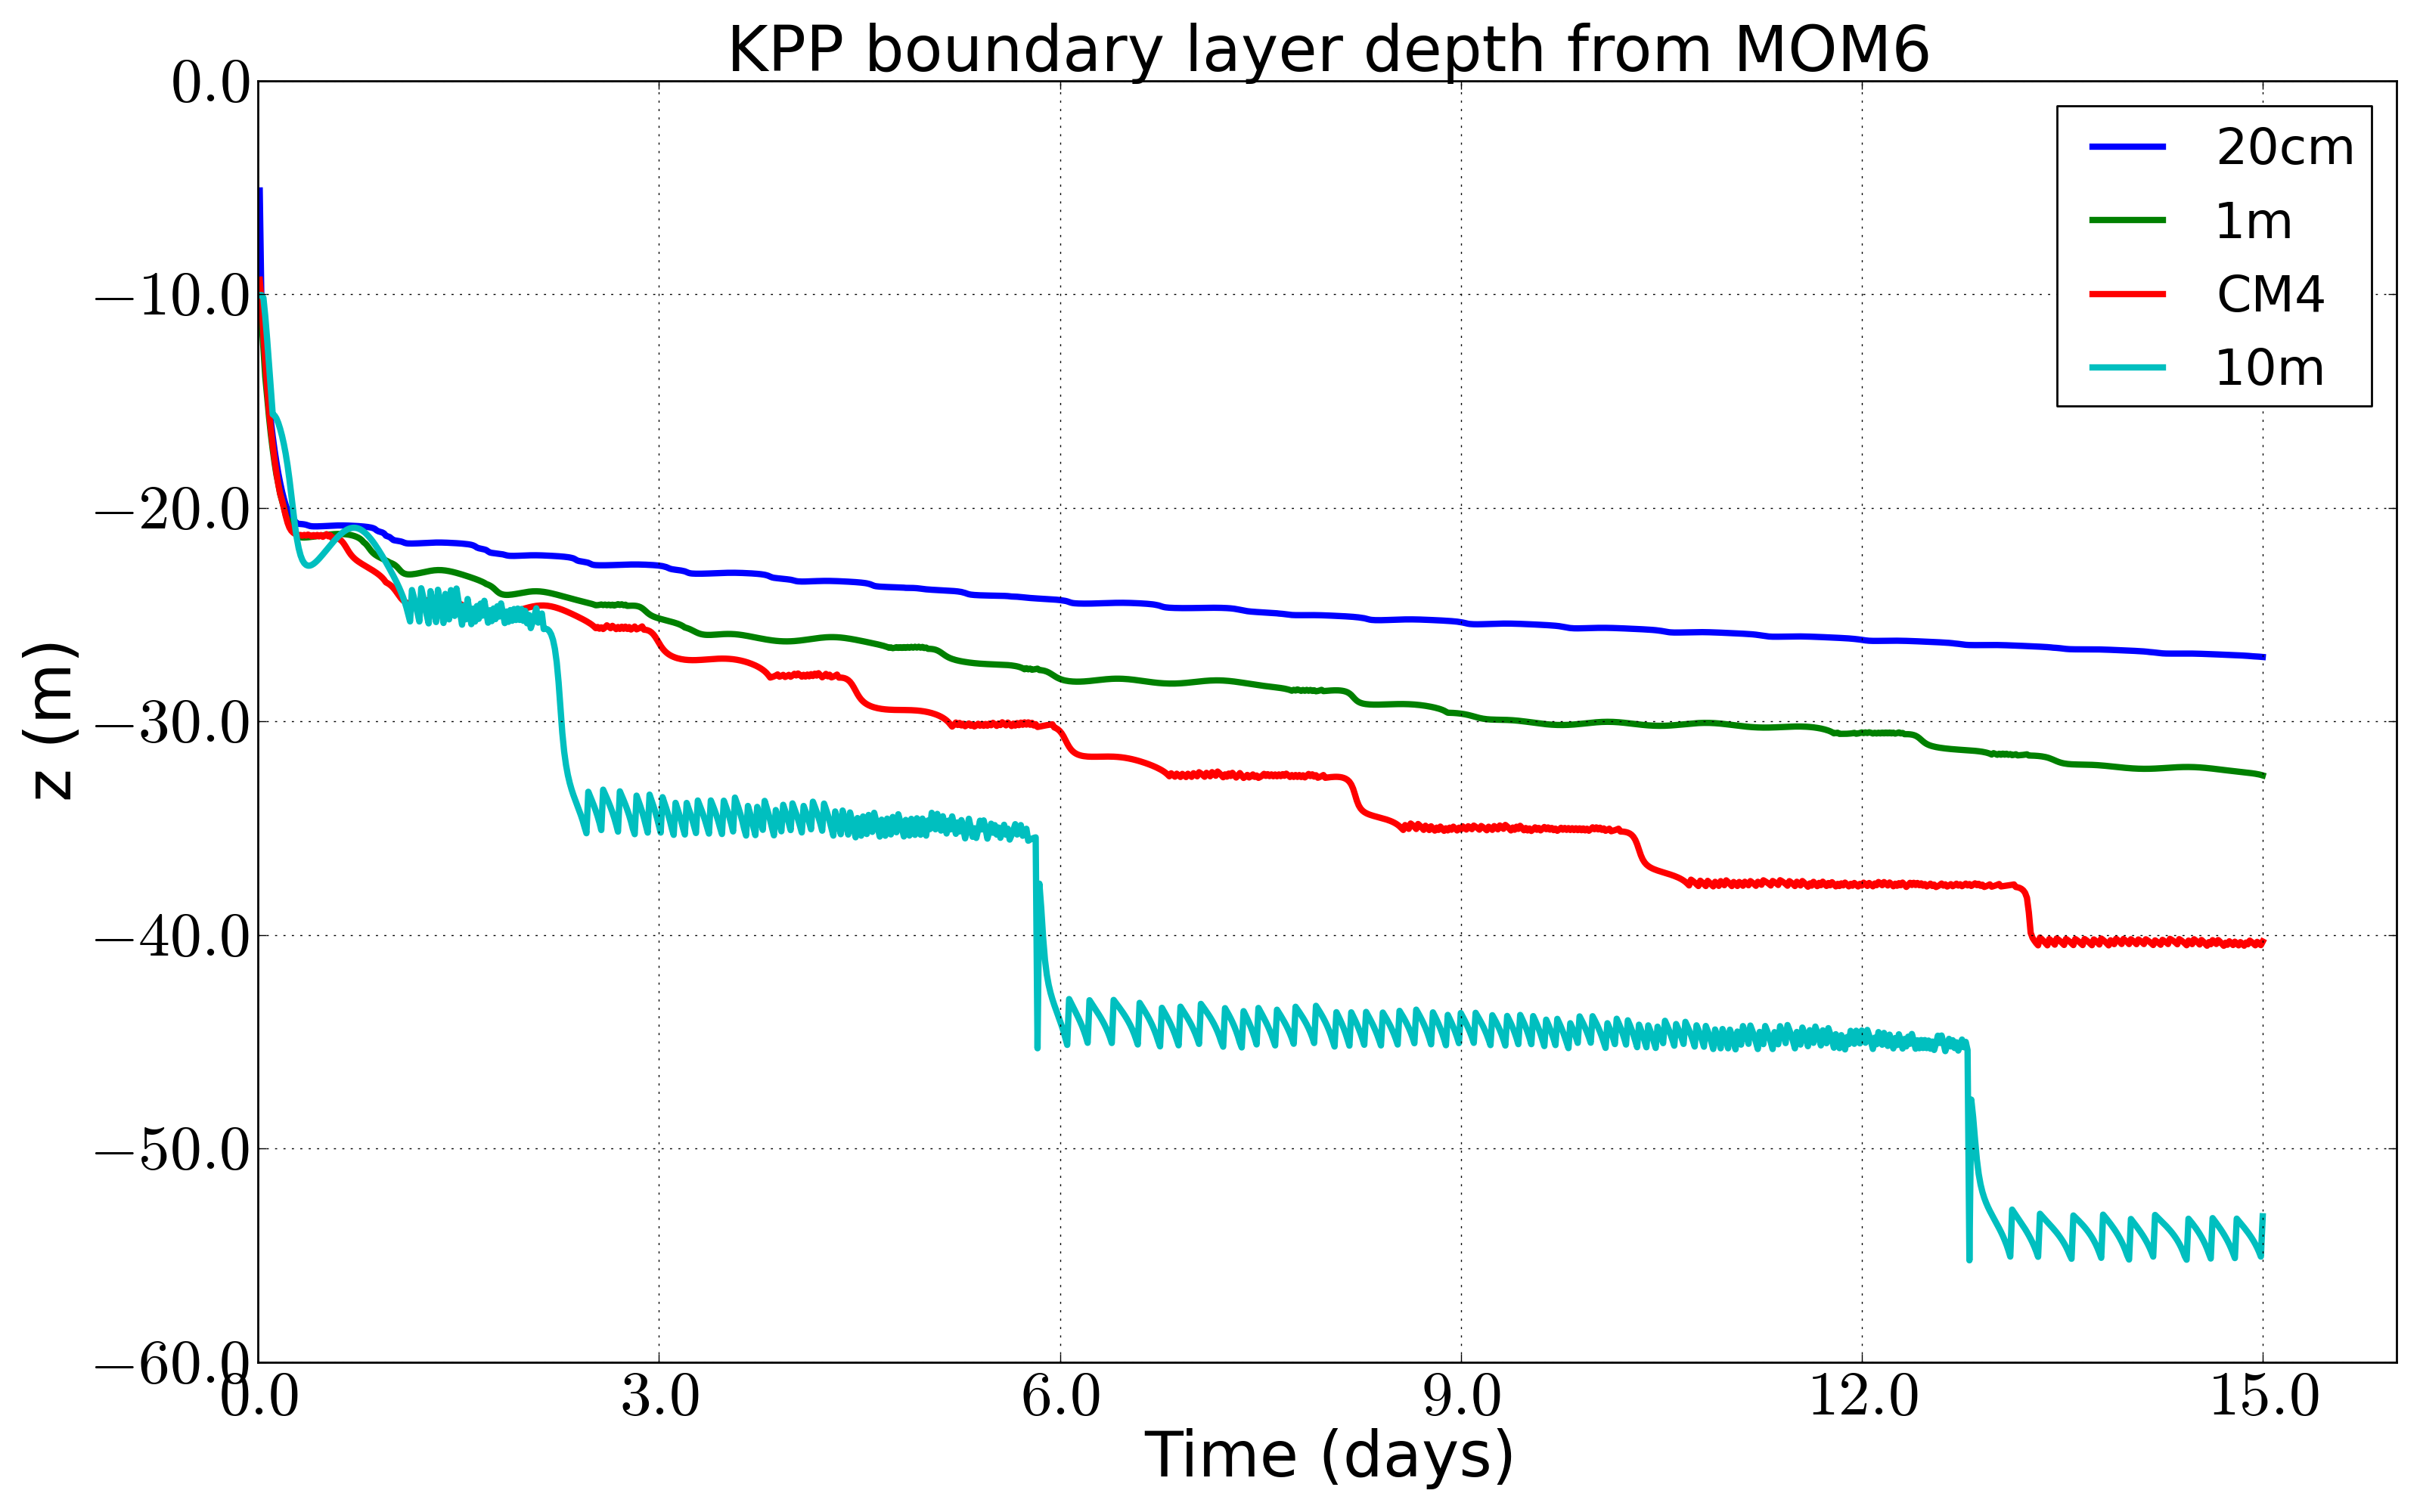
\includegraphics[angle=0,width=8cm]{./figs/MOM6/WSwPSBF_A_MOM6_KPP_bldepth.png}
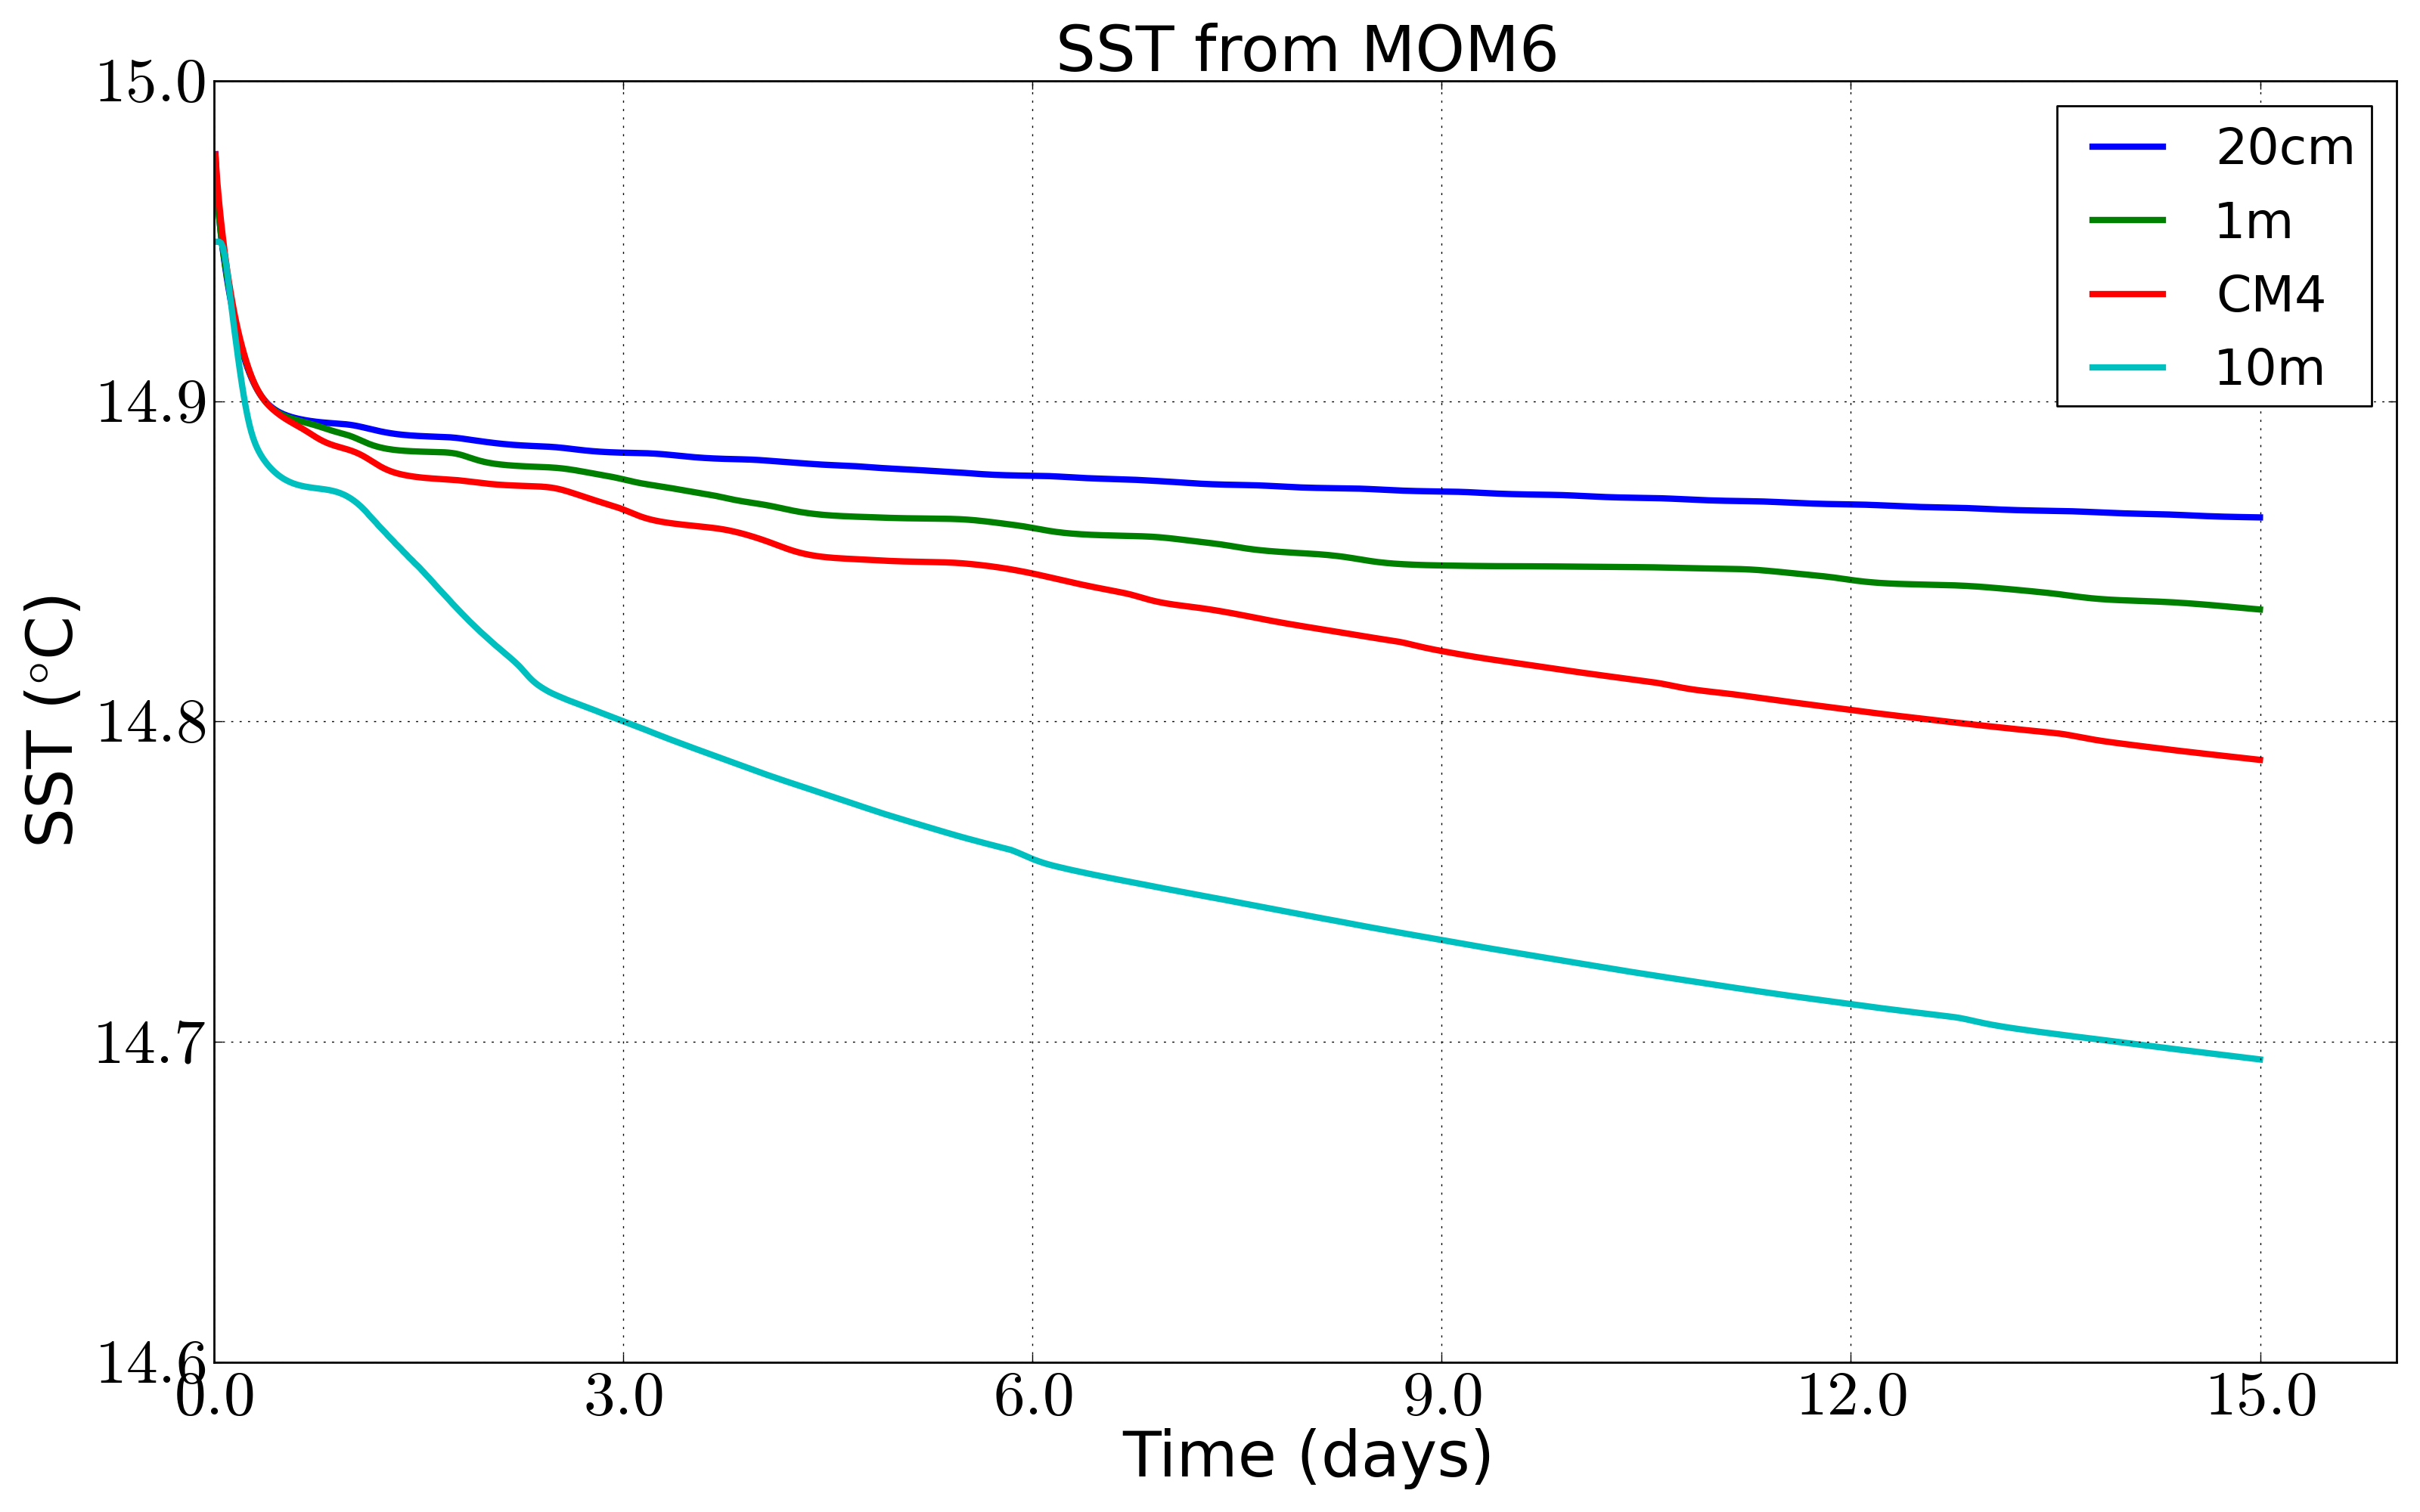
\includegraphics[angle=0,width=8cm]{./figs/MOM6/WSwPSBF_A_MOM6_SST.png}
\caption[KPP boundary layer depth and SST from MOM6 for WSwPSBF.A
]{\sf Time series for KPP boundary layer depth (left panel) and SST
  (right panel) for WSwPSBF.A (constant zonal wind stress and zero
  surface buoyancy forcing) as realized in MOM6.}
\label{fig:WSwPSBF_A_MOM6_SST_bldepth}
\end{center}
%\rule{\textwidth}{0.005in}
\end{figure}
%%%%%%%%%%%%%%%%%%%%%%%%%%%%%%%%%%%%%%%%%%%%%%%%%%%%%%%%%%%%%%%%%%%%%%%%


%%%%%%%%%%%%%%%%%%%% %%%%%%%%%%%%%%%%%%%%%%%%%
\begin{figure}[h!t]
%\rule{\textwidth}{0.005in}
\begin{center}
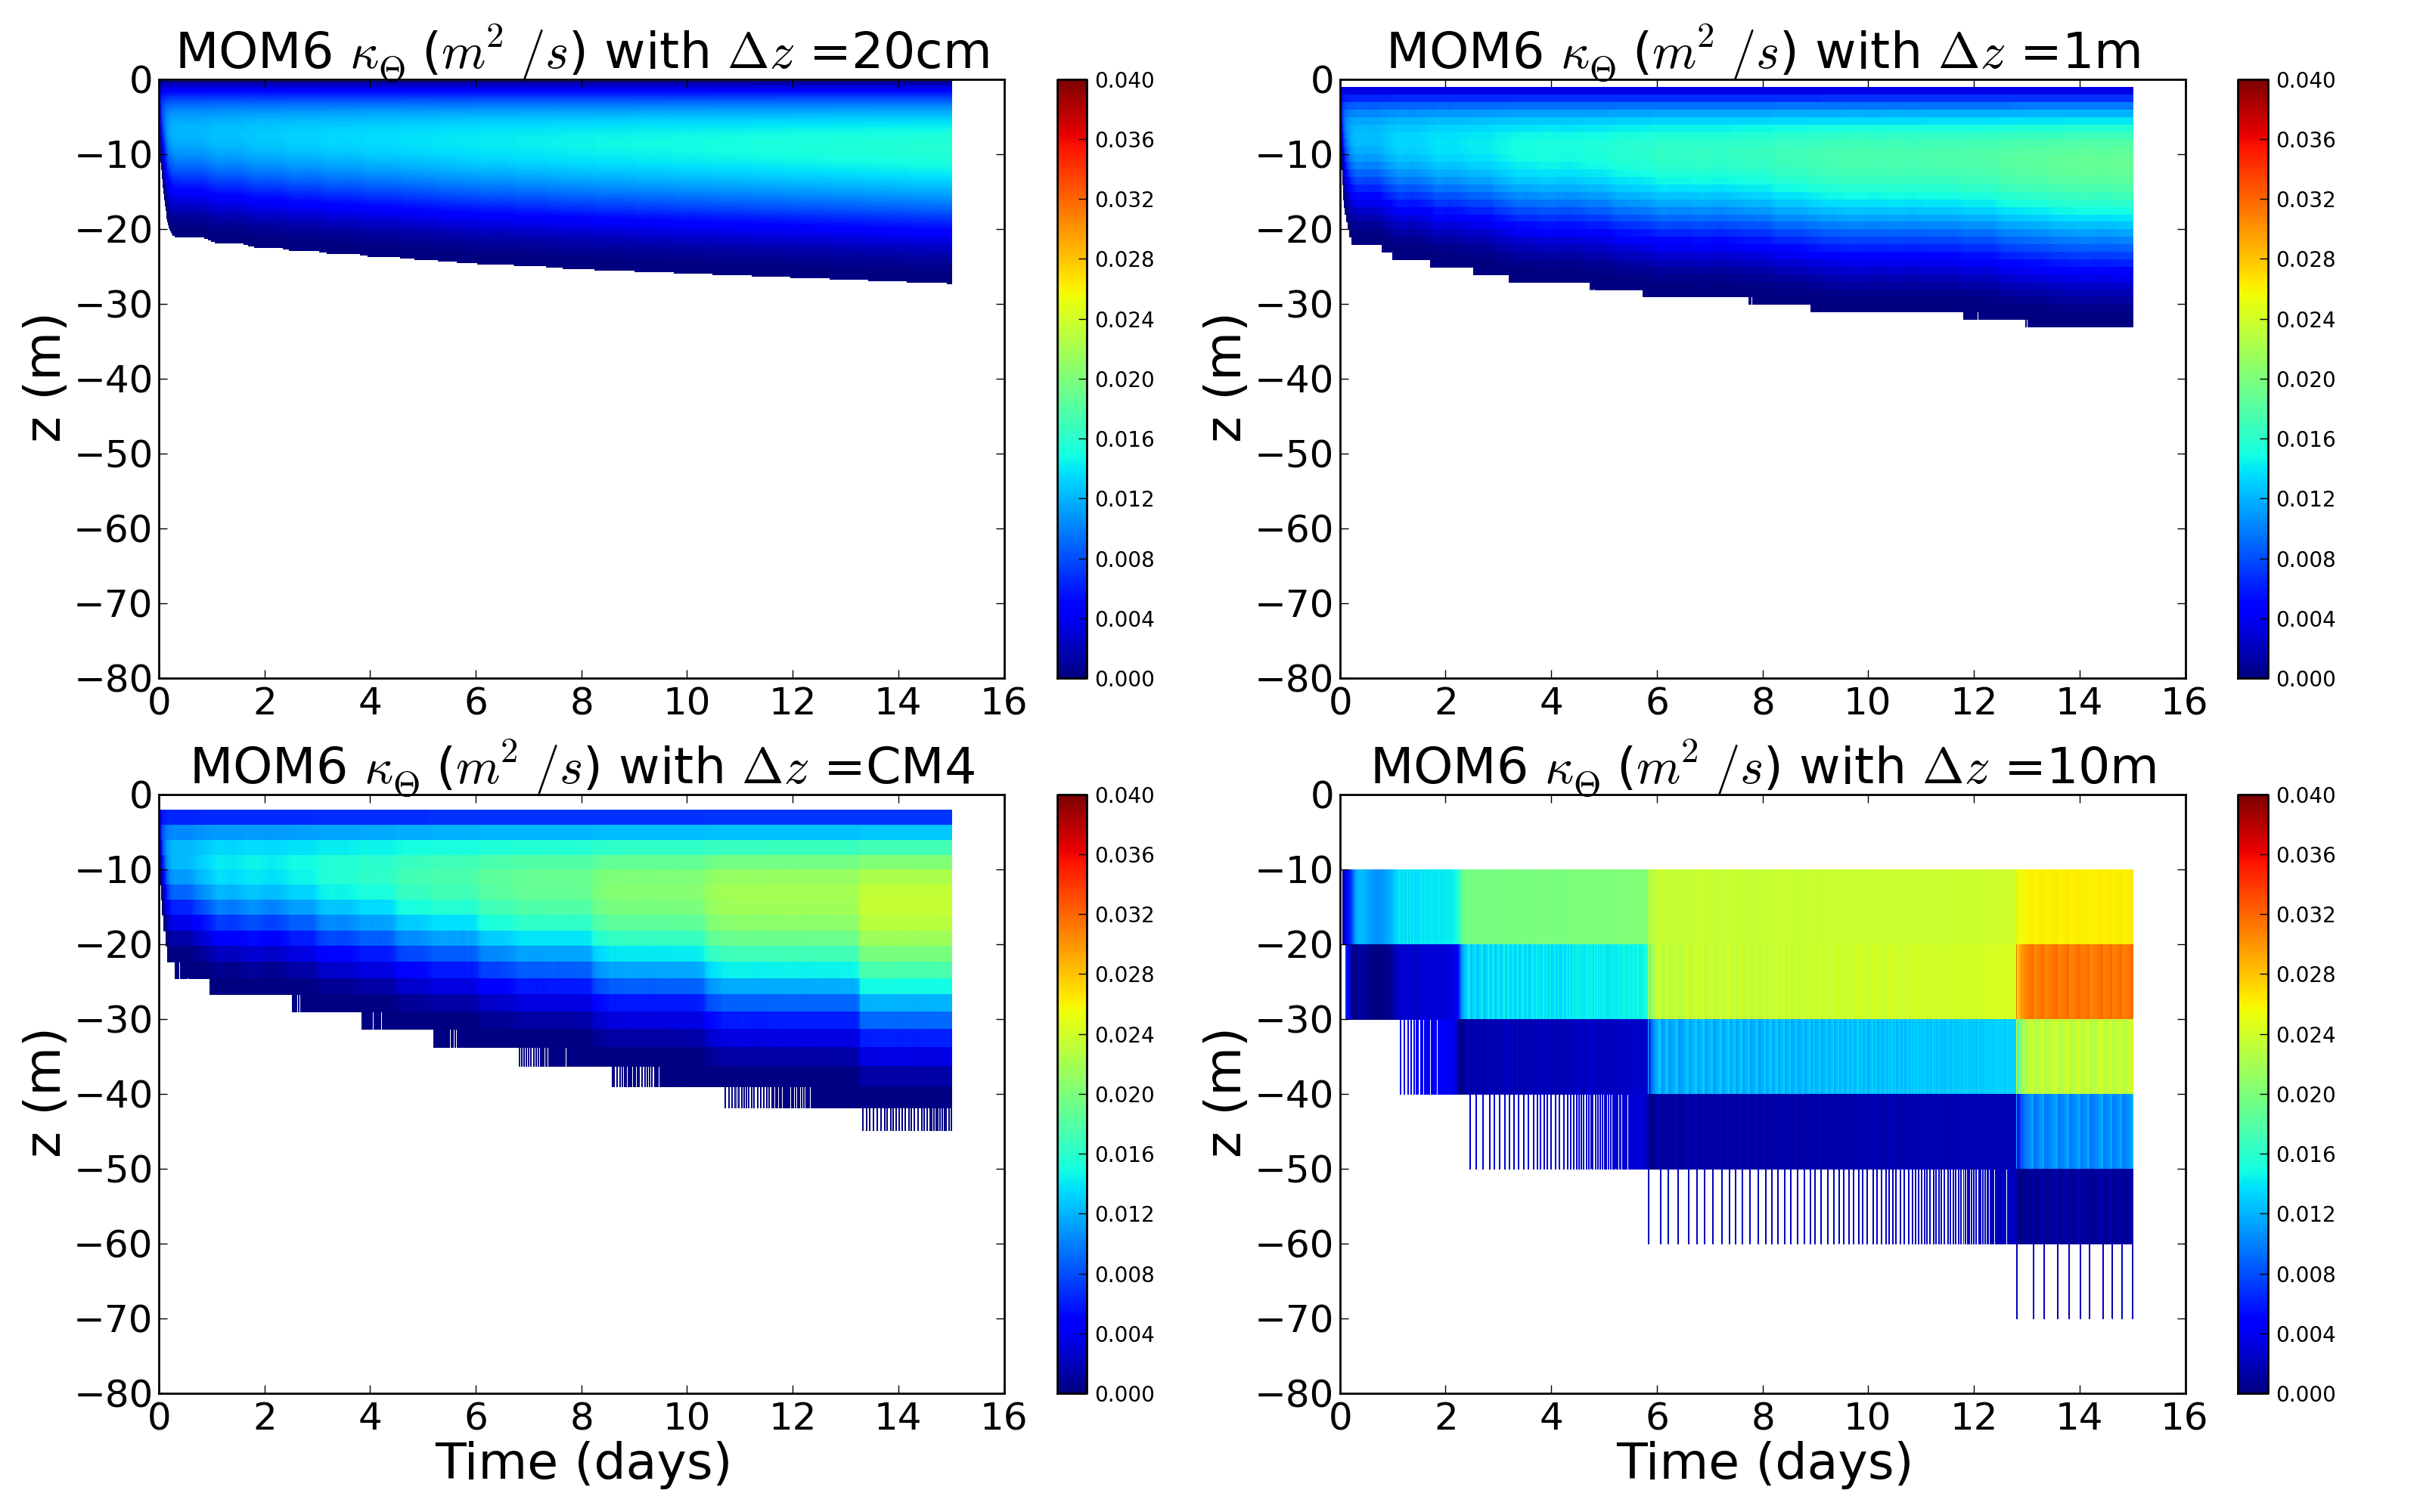
\includegraphics[angle=0,width=14cm]{./figs/MOM6/WSwPSBF_A_MOM6_KPP_diffusivity.png}
\caption[KPP diffusivity from MOM6 for WSwPSBF.A ]{\sf Time series for
  the KPP vertical diffusivity for WSwPSBF.A (constant zonal wind
  stress and zero surface buoyancy forcing) as realized in MOM6 using
  four different vertical grid resolutions.  The diffusivity is
  centered on the bottom interface of a grid cell, with the first
  nonzero value at the bottom of the surface cell.  The diffusivity
  vanishes one cell below the boundary layer: \color{red} why not at
  the boundary layer depth?  Do we always bias towards one cell
  deeper? \color{black}.}
\label{fig:WSwPSBF_A_MOM6_KPP_diffusivity}
\end{center}
%\rule{\textwidth}{0.005in}
\end{figure}
%%%%%%%%%%%%%%%%%%%%%%%%%%%%%%%%%%%%%%%%%%%%%%%%%%%%%%%%%%%%%%%%%%%%%%%%


%%%%%%%%%%%%%%%%%%%% %%%%%%%%%%%%%%%%%%%%%%%%%
\begin{figure}[h!t]
%\rule{\textwidth}{0.005in}
\begin{center}
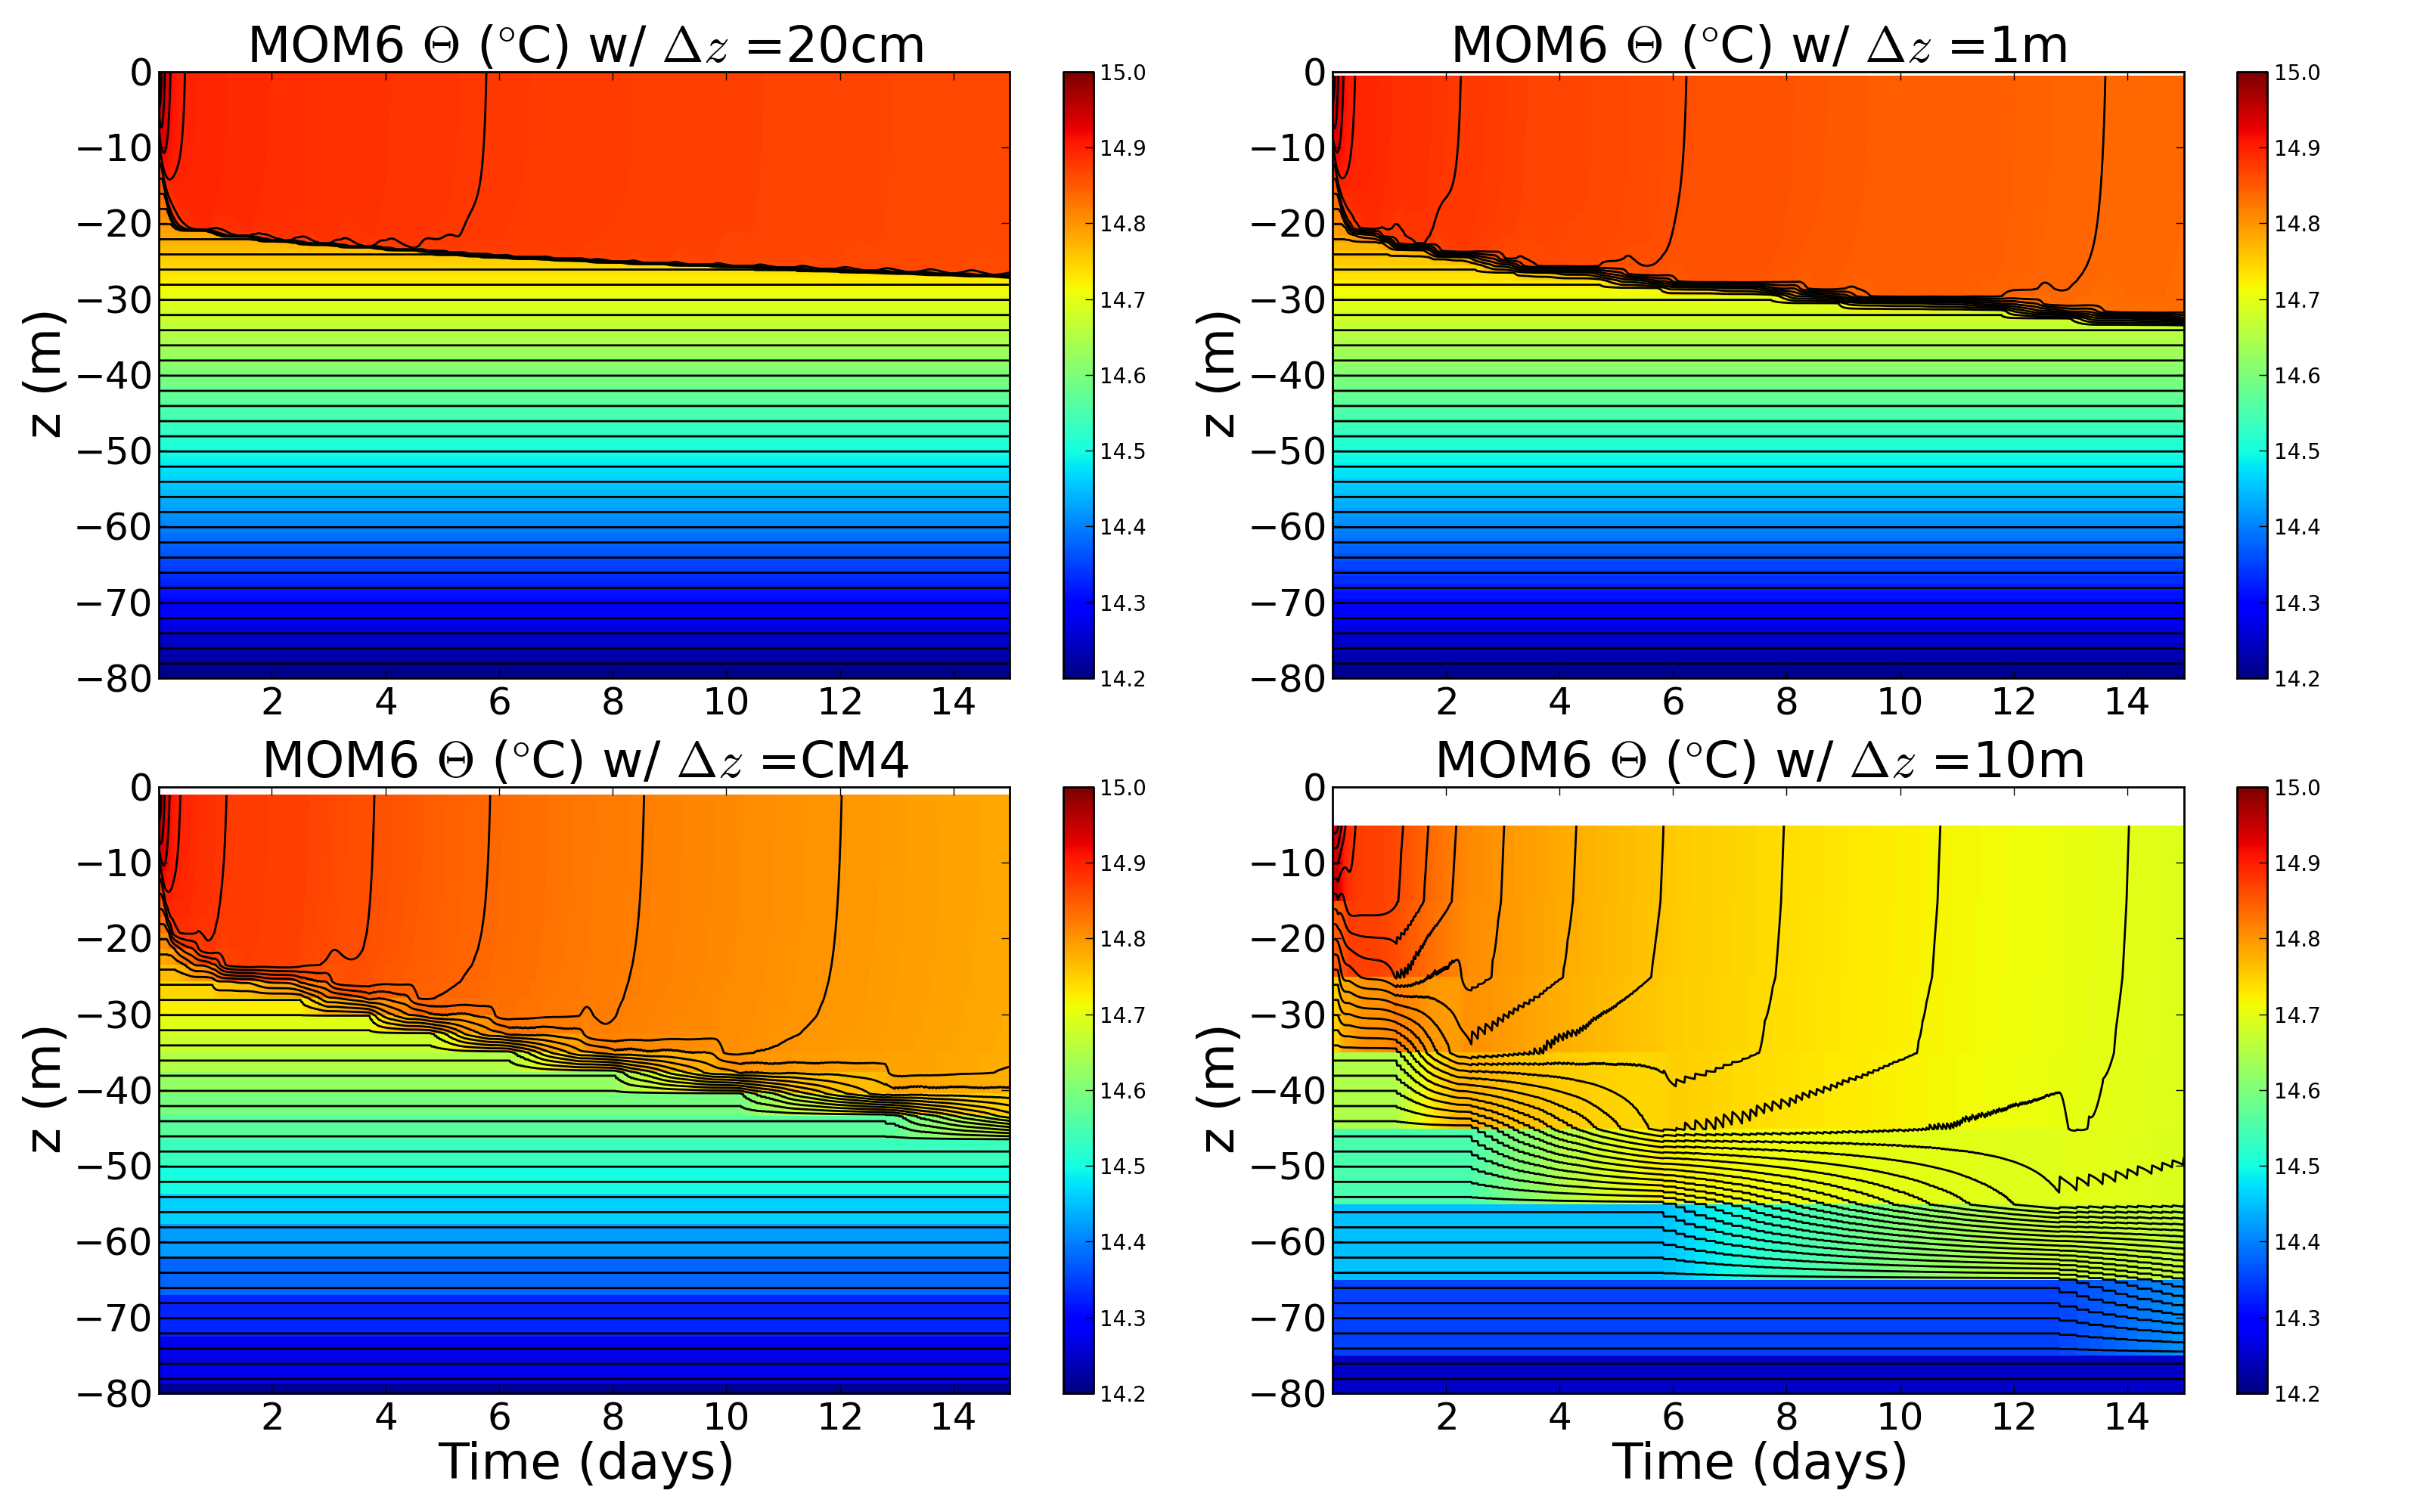
\includegraphics[angle=0,width=14cm]{./figs/MOM6/WSwPSBF_A_MOM6_temp.png}
\caption[Temperature from MOM6 for WSwPSBF.A ]{\sf Time series for
  temperature in the test case WSwPSBF.A (constant zonal wind stress
  and zero surface buoyancy forcing) as realized in MOM6 using four
  different vertical grid resolutions.  The temperature is centered on
  the center of a grid cell, with the first nonzero value at the
  center of the surface cell.}
\label{fig:WSwPSBF_A_MOM6_temp}
\end{center}
%\rule{\textwidth}{0.005in}
\end{figure}
%%%%%%%%%%%%%%%%%%%%%%%%%%%%%%%%%%%%%%%%%%%%%%%%%%%%%%%%%%%%%%%%%%%%%%%%

%%%%%%%%%%%%%%%%%%%% %%%%%%%%%%%%%%%%%%%%%%%%%
\begin{figure}[h!t]
%\rule{\textwidth}{0.005in}
\begin{center}
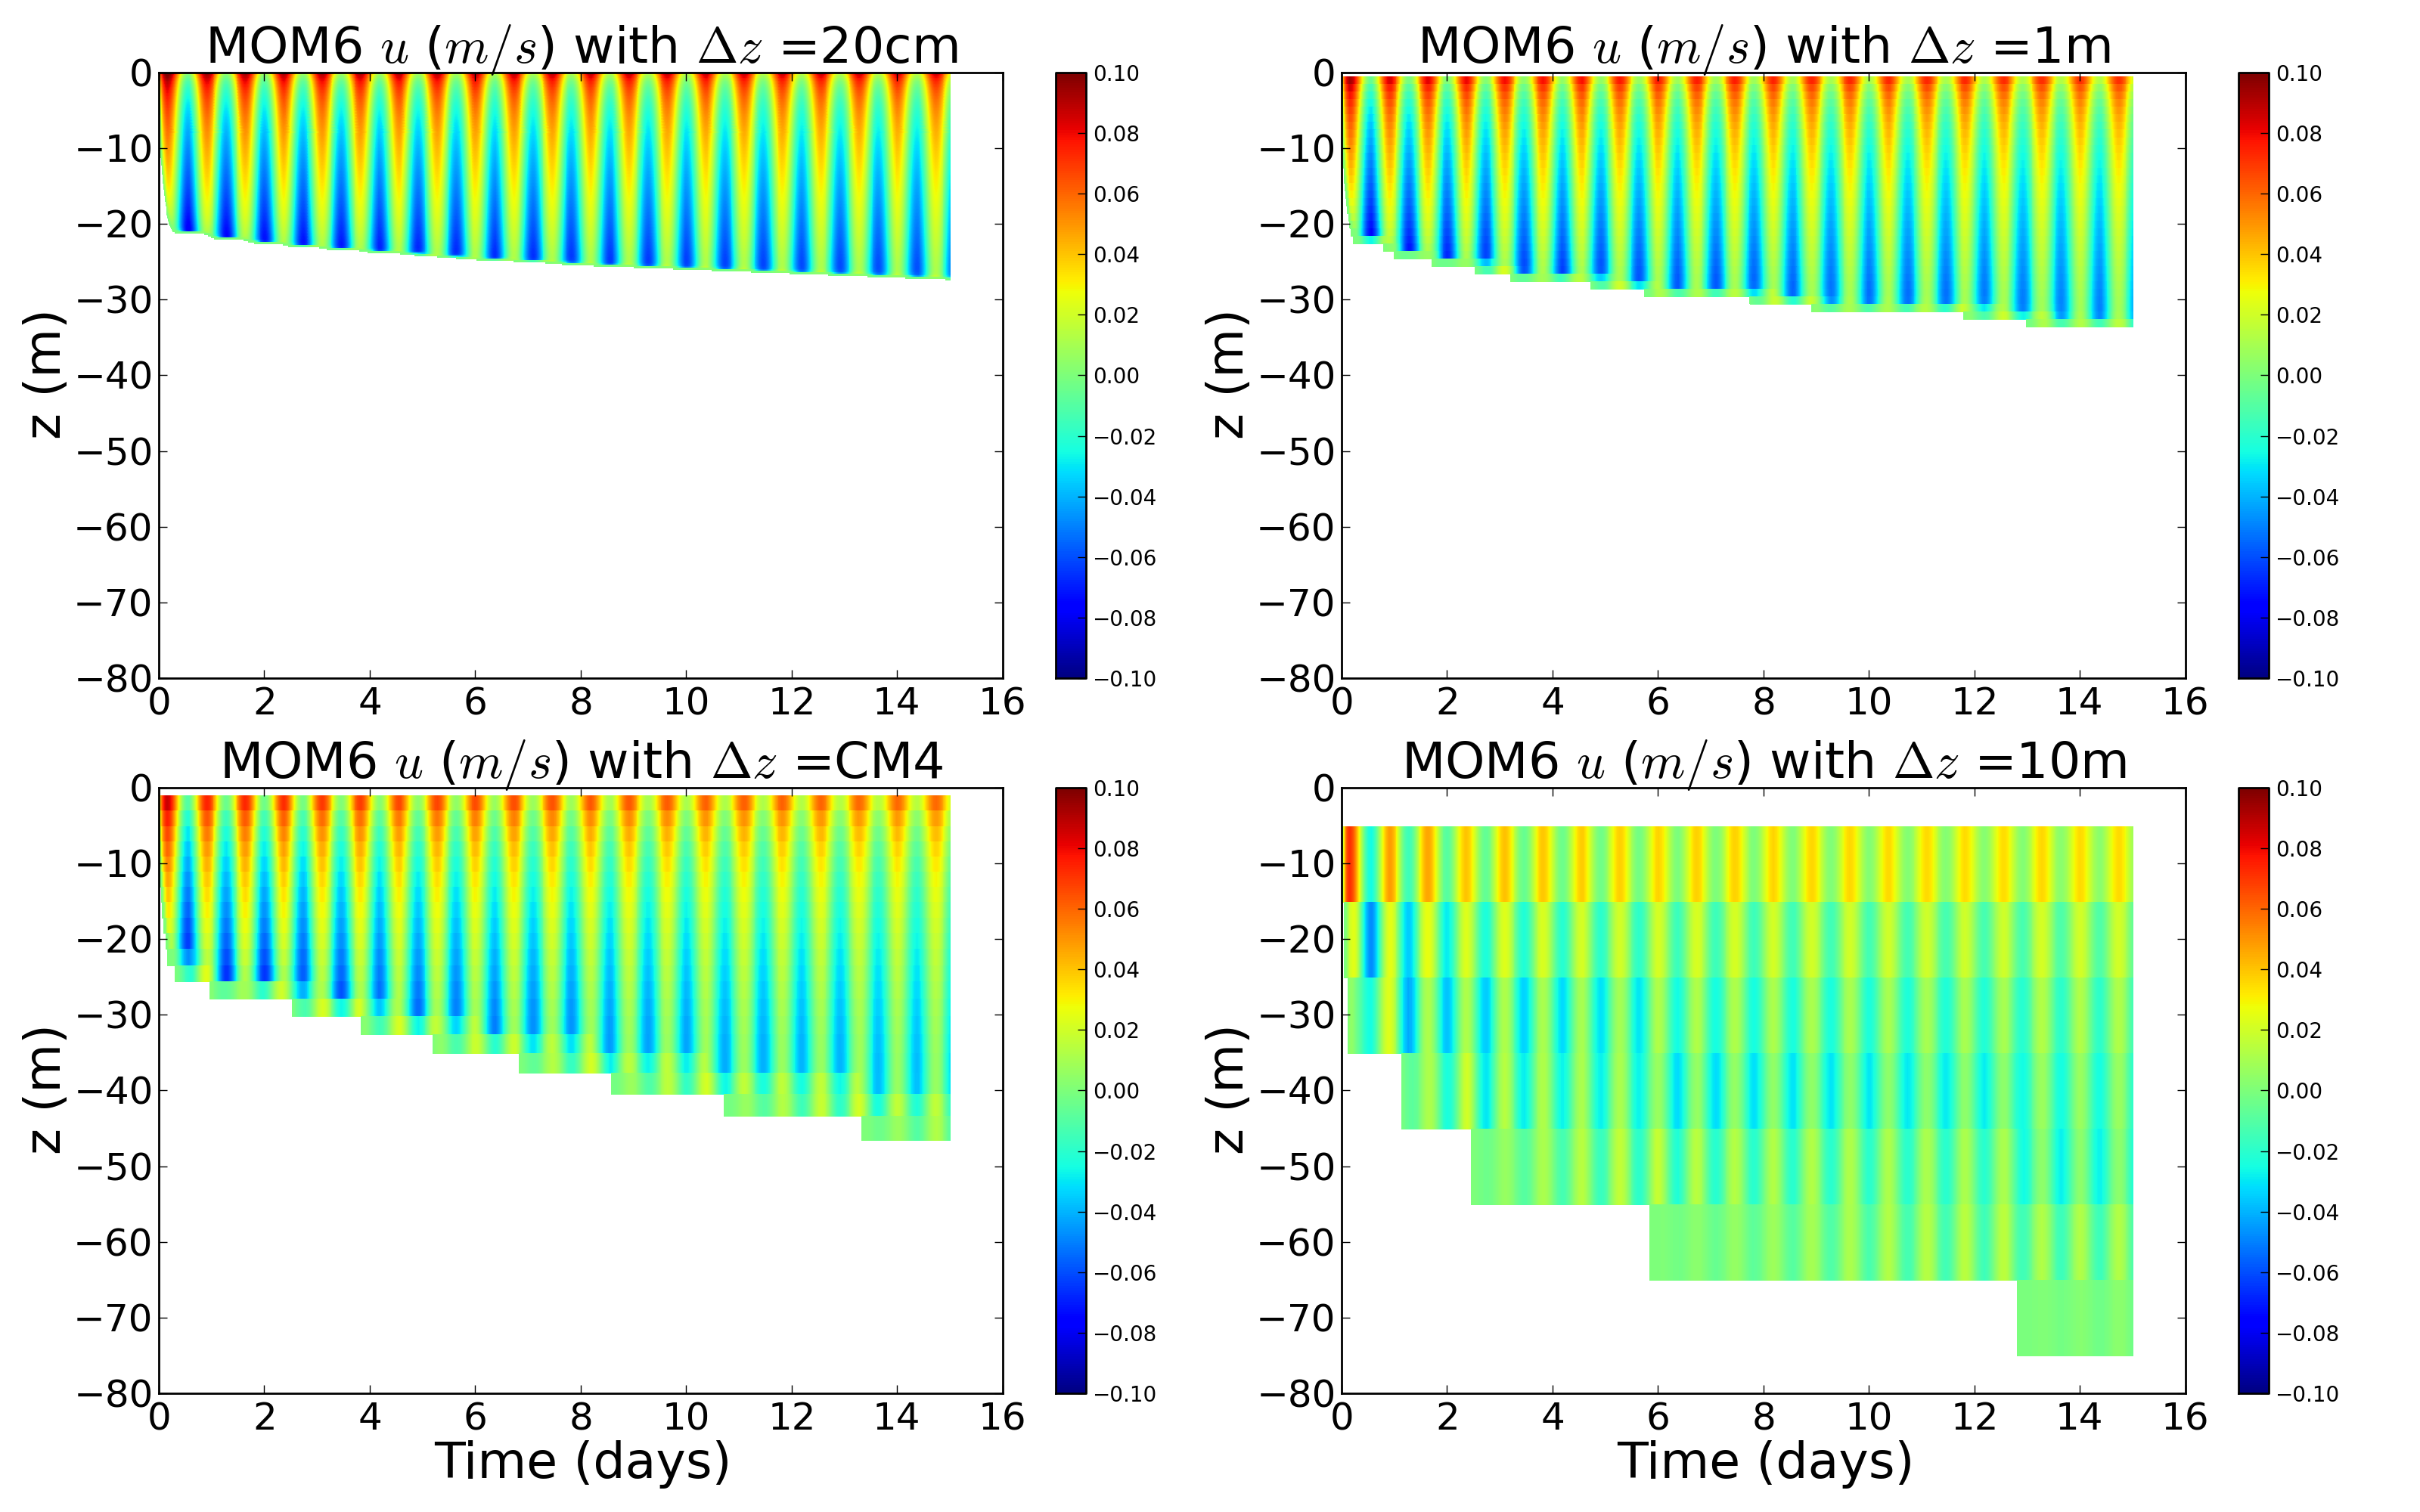
\includegraphics[angle=0,width=14cm]{./figs/MOM6/WSwPSBF_A_MOM6_zonal_velocity.png}
\caption[Zonal velocity from MOM6 for WSwPSBF.A ]{\sf Time series for
  zonal velocity in the test case WSwPSBF.A (constant zonal wind
  stress and zero surface buoyancy forcing) as realized in MOM6 using
  four different vertical grid resolutions. The velocity is centered
  on the center of a grid cell, with the first nonzero value at the
  center of the surface cell.}
\label{fig:WSwPSBF_A_MOM6_zonal}
\end{center}
%\rule{\textwidth}{0.005in}
\end{figure}
%%%%%%%%%%%%%%%%%%%%%%%%%%%%%%%%%%%%%%%%%%%%%%%%%%%%%%%%%%%%%%%%%%%%%%%%



\clearpage 


\section{Results for WSwPSBF.B $(Q=100~\mbox{W}~\mbox{m}^{-2})$}
\label{section:WSwPSBFB}

We here present results from the three ocean models for the experiment
WSwPSBF.B, in which there is a constant surface heat flux of
$Q=100~\mbox{W}~\mbox{m}^{-2}$ along with the constant zonal wind
stress $\tau^{x} = 0.1~\mbox{N}~\mbox{m}^{-2}$.  Mixing occurs only
through mechanical forcing from the wind stress.  Given the positive
buoyancy forcing in this test, the boundary layer does not deepen as
much as in test WSwPSBF.A discussed in Section \ref{section:WSwPSBFA}.
This test exhibits less sensitivity to vertical grid spacing than
WSwPSBF.A.  


\subsection{GFDL-MOM6} 

Figure \ref{fig:WSwPSBF_B_MOM6_SST_bldepth} shows the KPP boundary
layer depth from the MOM6 implementation of CVMix.  The boundary layer
rapidly deepens to roughly $18~\mbox{m}$, and then remains nearly for
most of the 15 day simulation.  There is a notable oscillation of the
boundary layer depth in the coarsest resolution with $\Delta z =
10~\mbox{m}$, whereas the other grids show relatively steady values by
roughly three days.  The oscillations have an inertial period of
roughly $0.73~\mbox{days}$ (equation (\ref{eq:inertial-period})).
After a couple of days, the SST steadily rises from the positive
surface heat flux, which dominates over the effects of wind mixing.

The SST is cooler with the coarsest grid $\Delta z = 10~\mbox{m}$.
The reason is that with this grid, the first non-zero KPP diffusivity
occurs at the bottom interface of the surface cell, which is at
$10~\mbox{m}$ depth (see Figure
\ref{fig:WSwPSBF_B_MOM6_KPP_diffusivity}).  This cell reaches into the
cooler interior more than the finer grids, and thus brings the surface
cell into contact with relatively cool interior waters.  Additionally,
note how the KPP diffusivity with $\Delta z = 10~\mbox{m}$ exhibits an
oscillatory behaviour, reflecting the inertial oscillations in the
boundary layer depth for this resolution.  Figure
\ref{fig:WSwPSBF_B_MOM6_temp} shows impacts of the upper ocean heating
on the depth profile of temperature, Figure
\ref{fig:WSwPSBF_B_MOM6_zonal} exhibits inertial oscillations in zonal
velocity associated with the zonal wind stress.

%%%%%%%%%%%%%%%%%%%% %%%%%%%%%%%%%%%%%%%%%%%%%
\begin{figure}[h!t]
%\rule{\textwidth}{0.005in}
\begin{center}
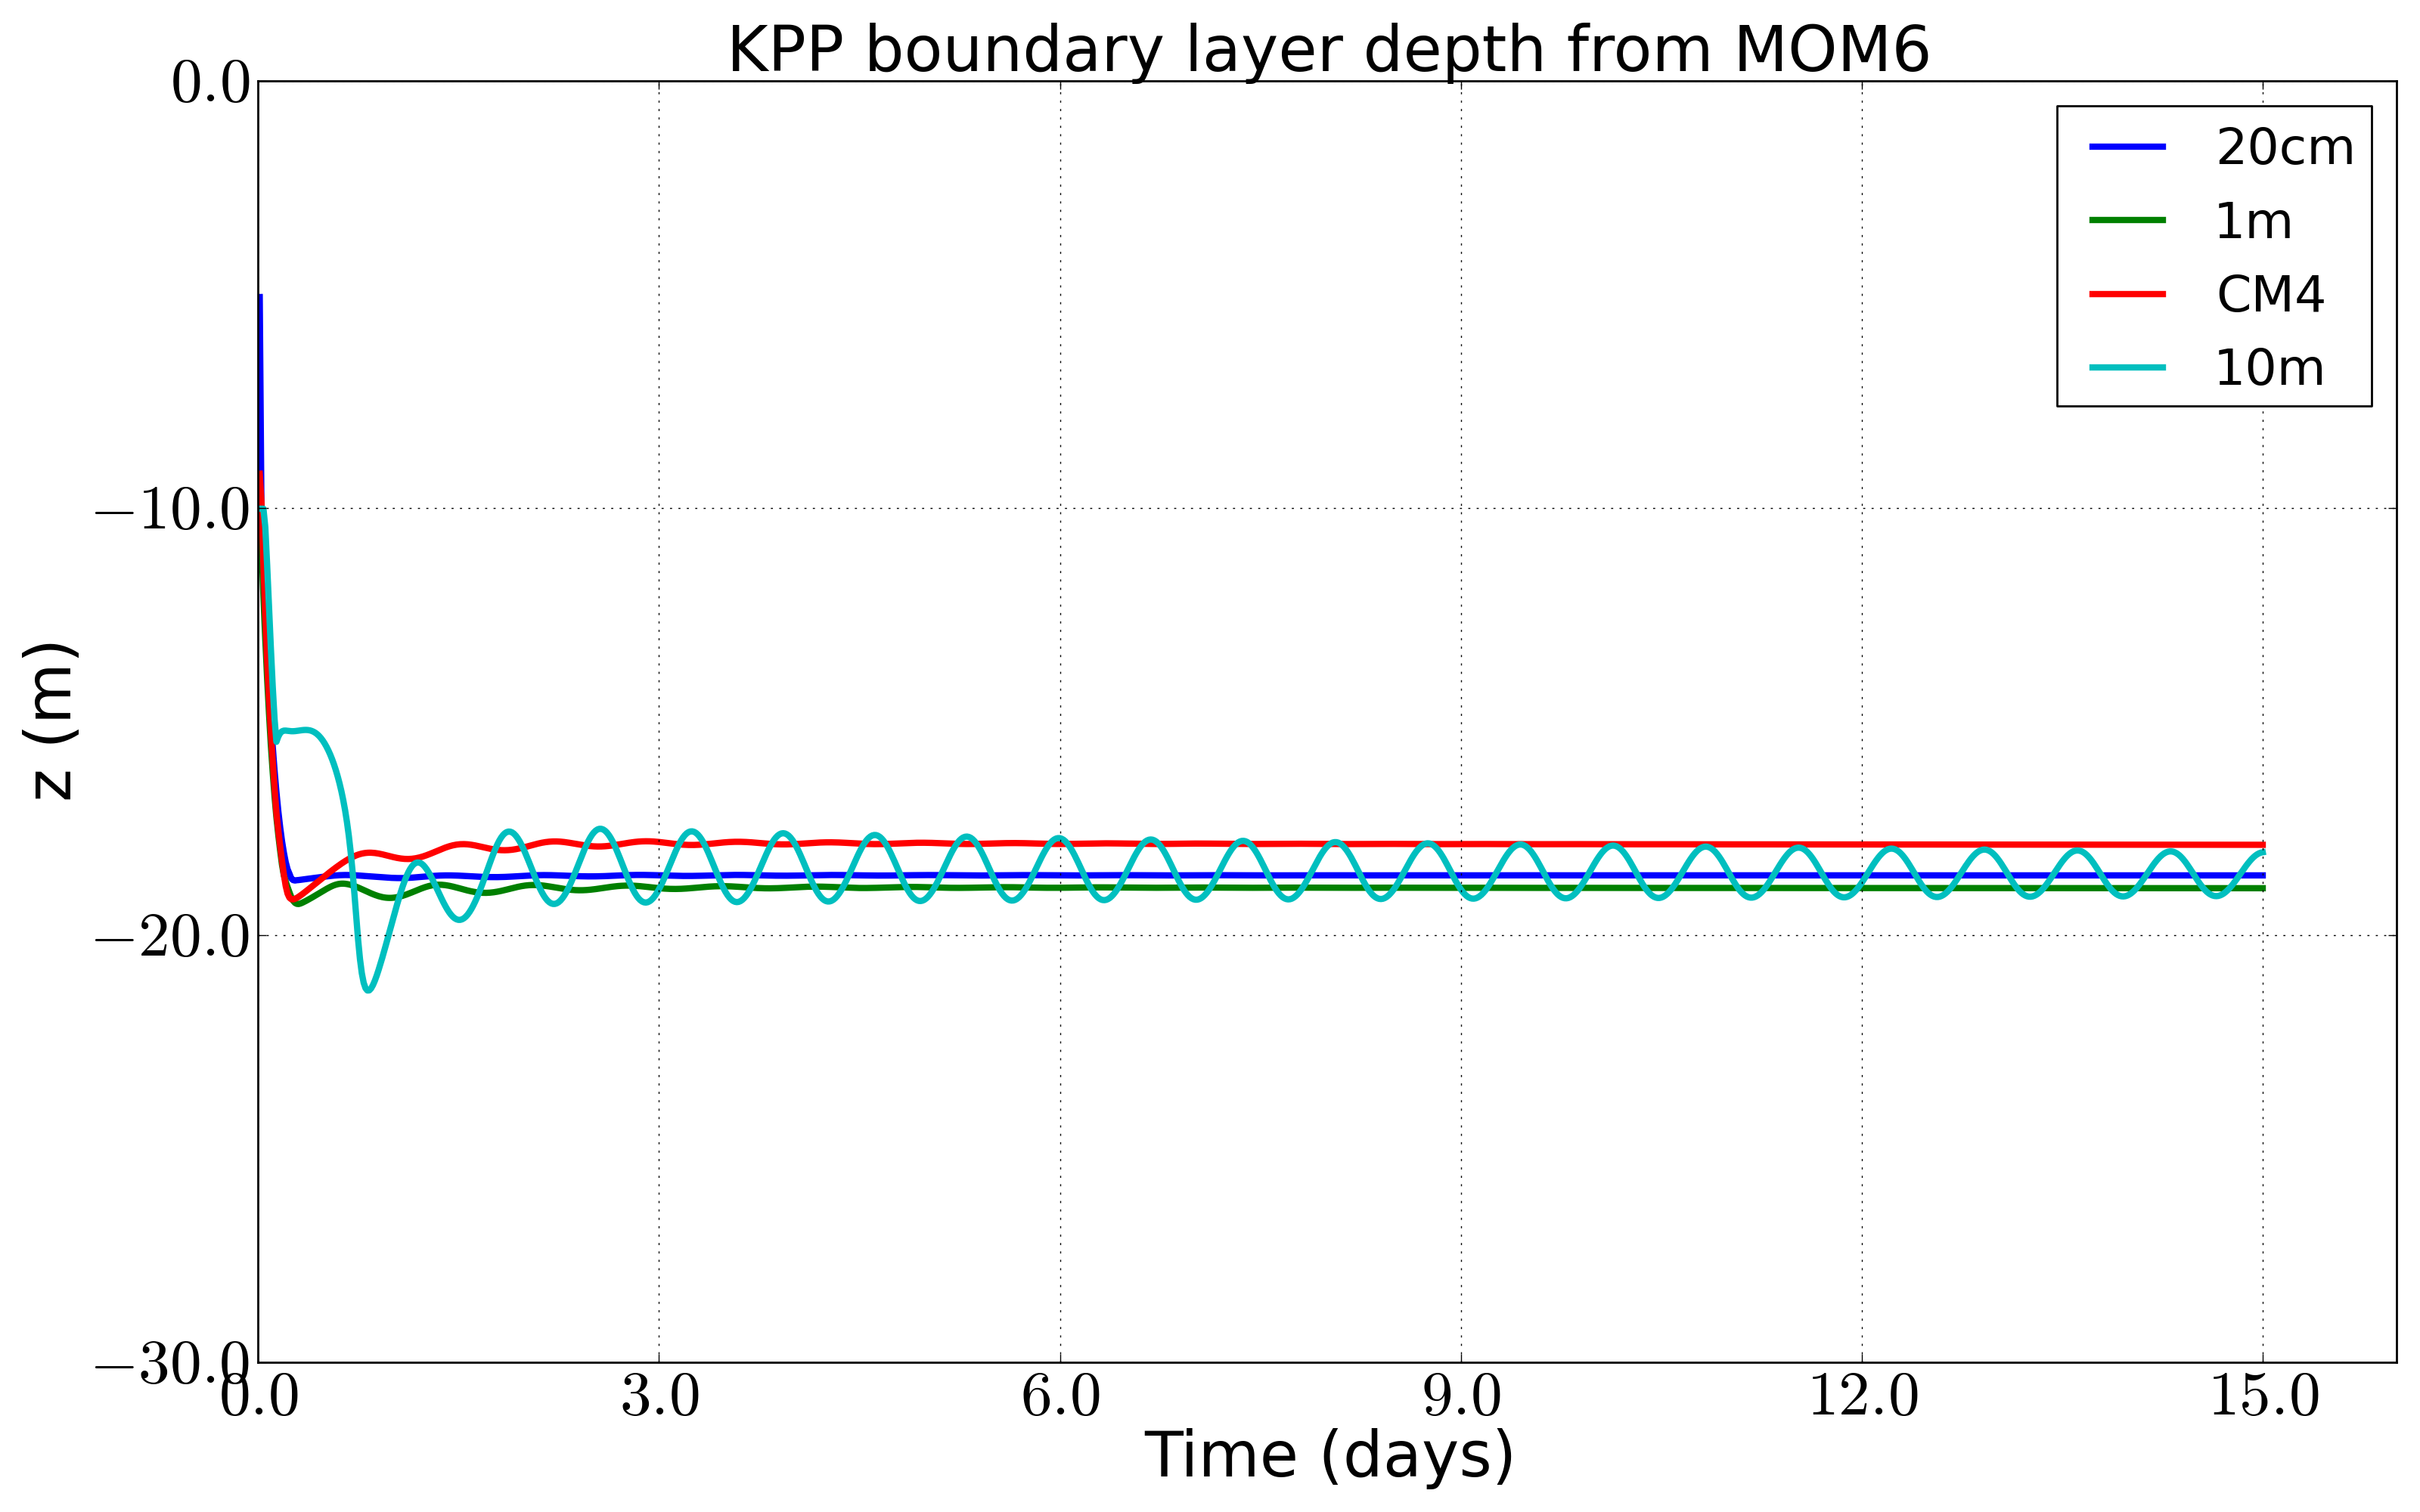
\includegraphics[angle=0,width=8cm]{./figs/MOM6/WSwPSBF_B_MOM6_KPP_bldepth.png}
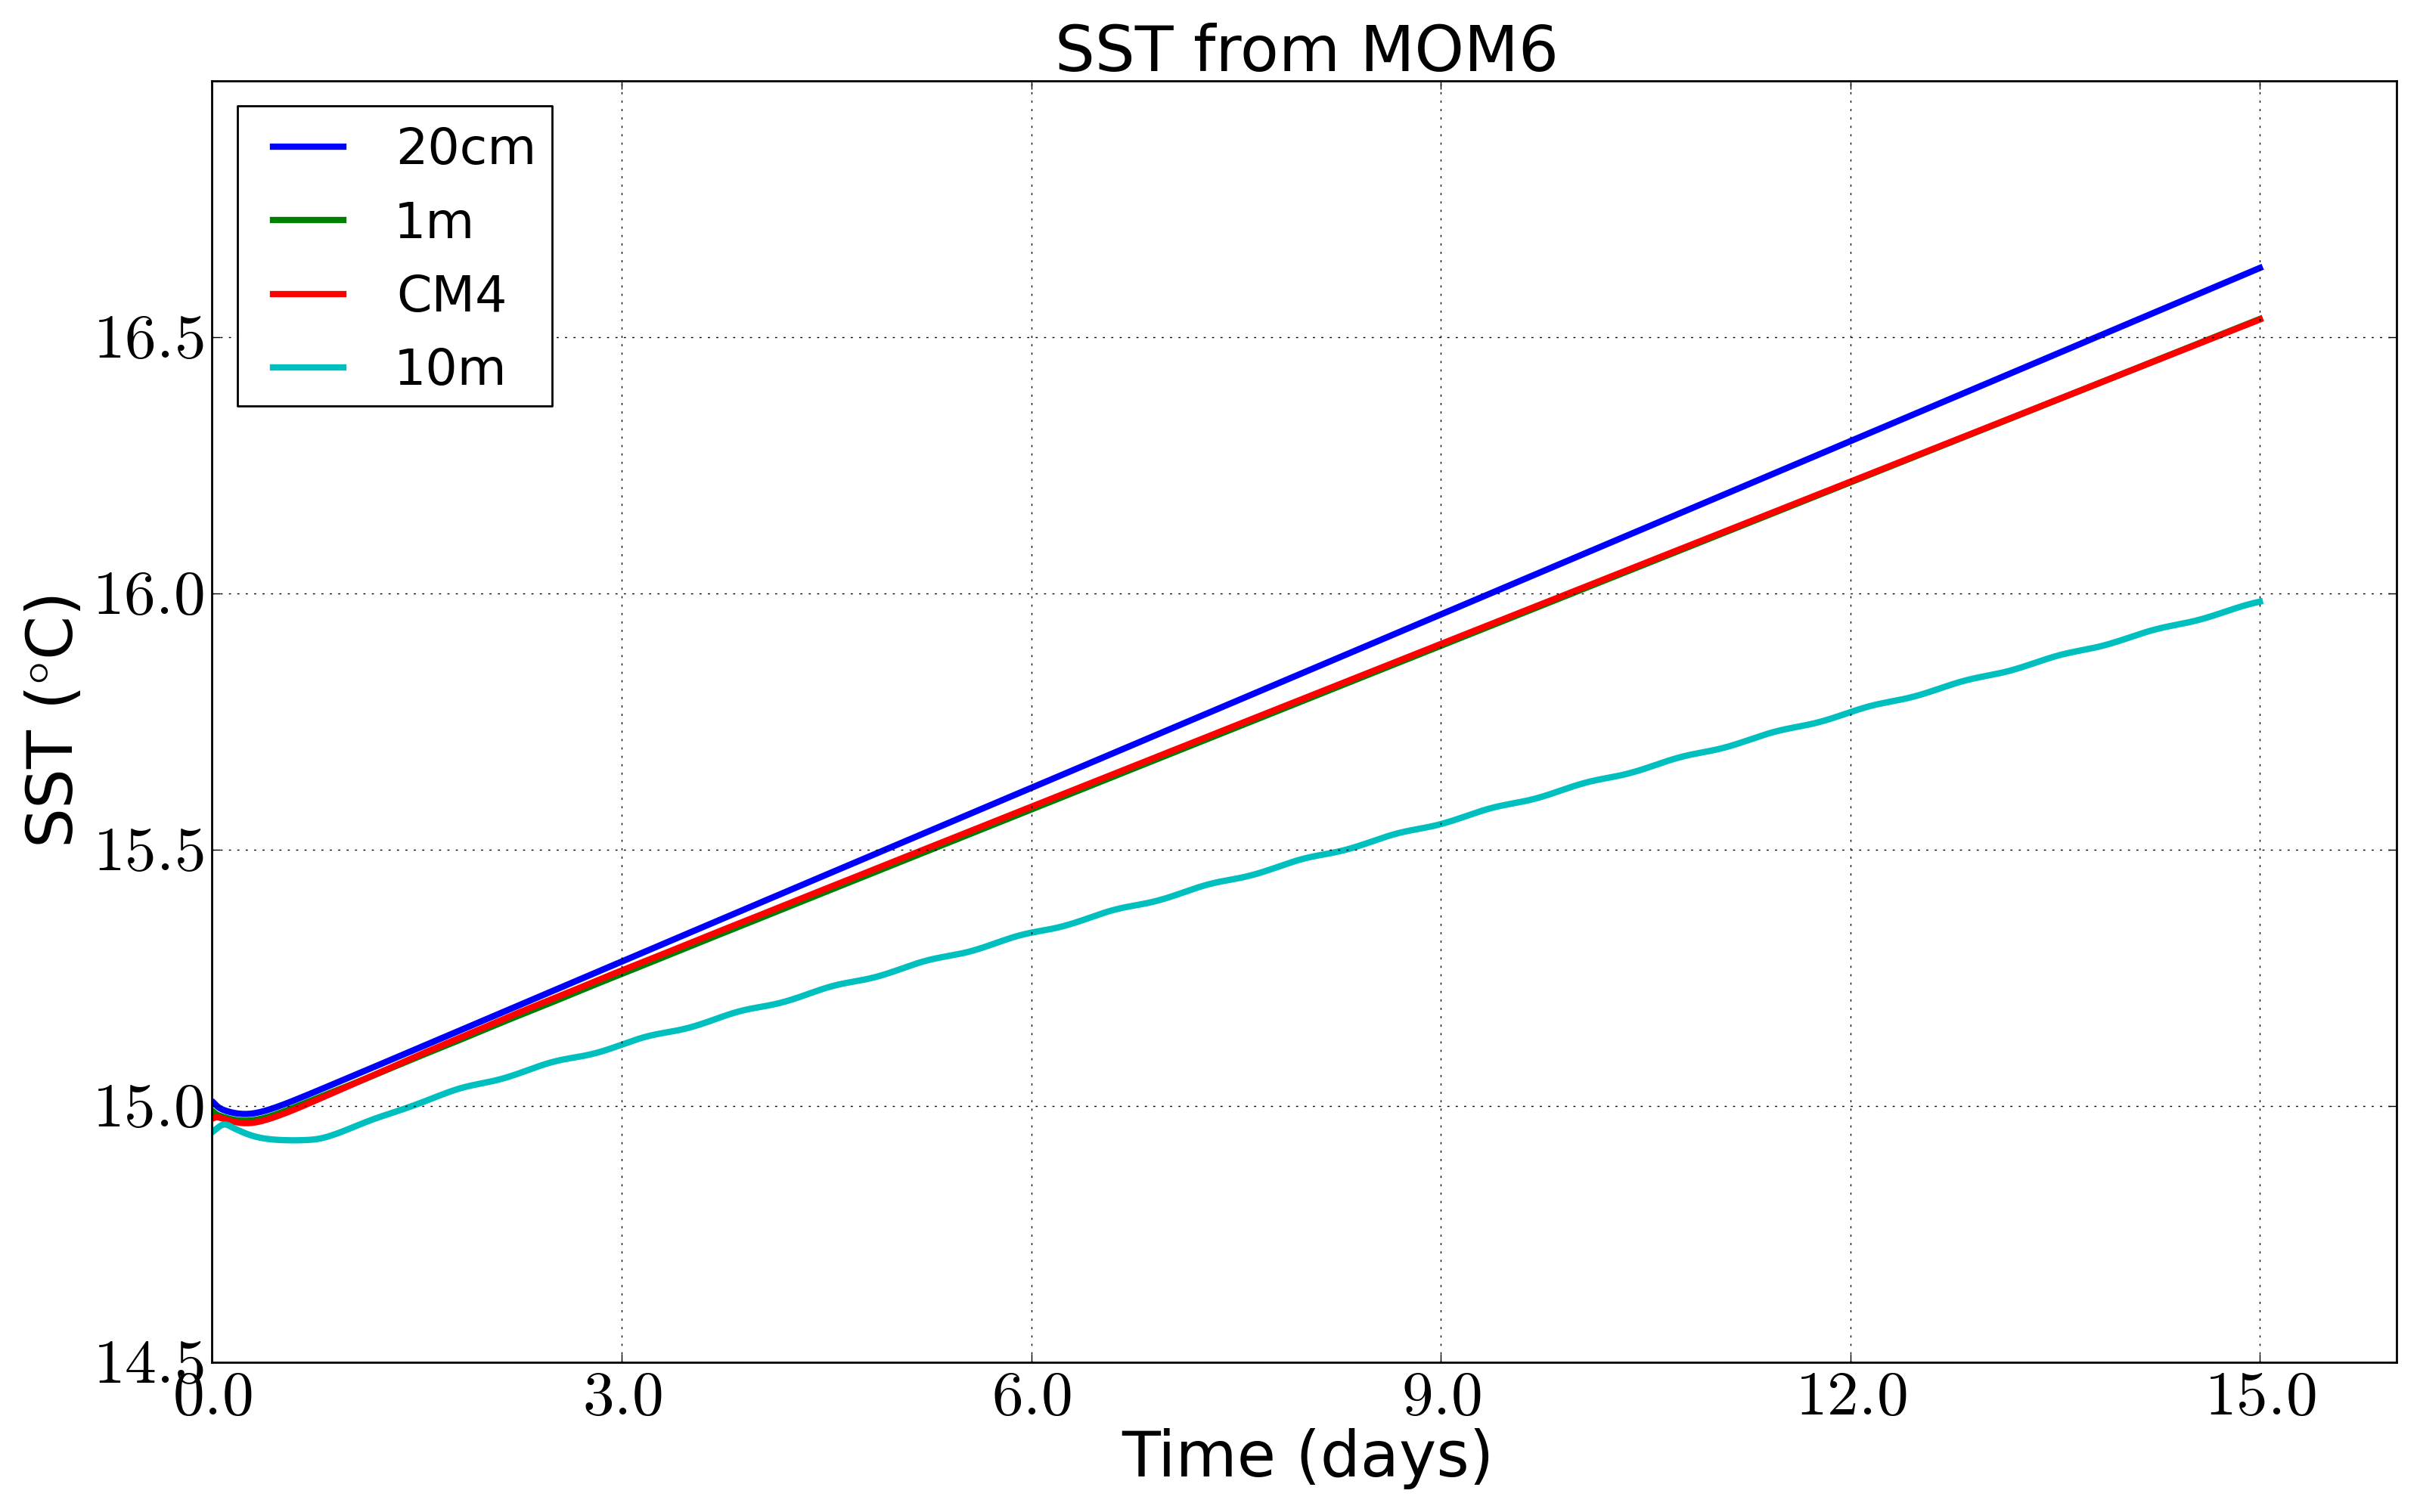
\includegraphics[angle=0,width=8cm]{./figs/MOM6/WSwPSBF_B_MOM6_SST.png}
\caption[KPP boundary layer depth and SST from MOM6 for WSwPSBF.B]
{\sf Time series for KPP boundary layer depth (left panel) and SST
  (right panel) for WSwPSBF.B (constant zonal wind stress and
  $Q=100~\mbox{W}~\mbox{m}^{-2}$) as realized in MOM6.  Note that SST
  for the $\Delta z = 1~\mbox{m}$ grid closely overlays that for the
  CM4 grid.}
\label{fig:WSwPSBF_B_MOM6_SST_bldepth}
\end{center}
%\rule{\textwidth}{0.005in}
\end{figure}
%%%%%%%%%%%%%%%%%%%%%%%%%%%%%%%%%%%%%%%%%%%%%%%%%%%%%%%%%%%%%%%%%%%%%%%%


%%%%%%%%%%%%%%%%%%%% %%%%%%%%%%%%%%%%%%%%%%%%%
\begin{figure}[h!t]
%\rule{\textwidth}{0.005in}
\begin{center}
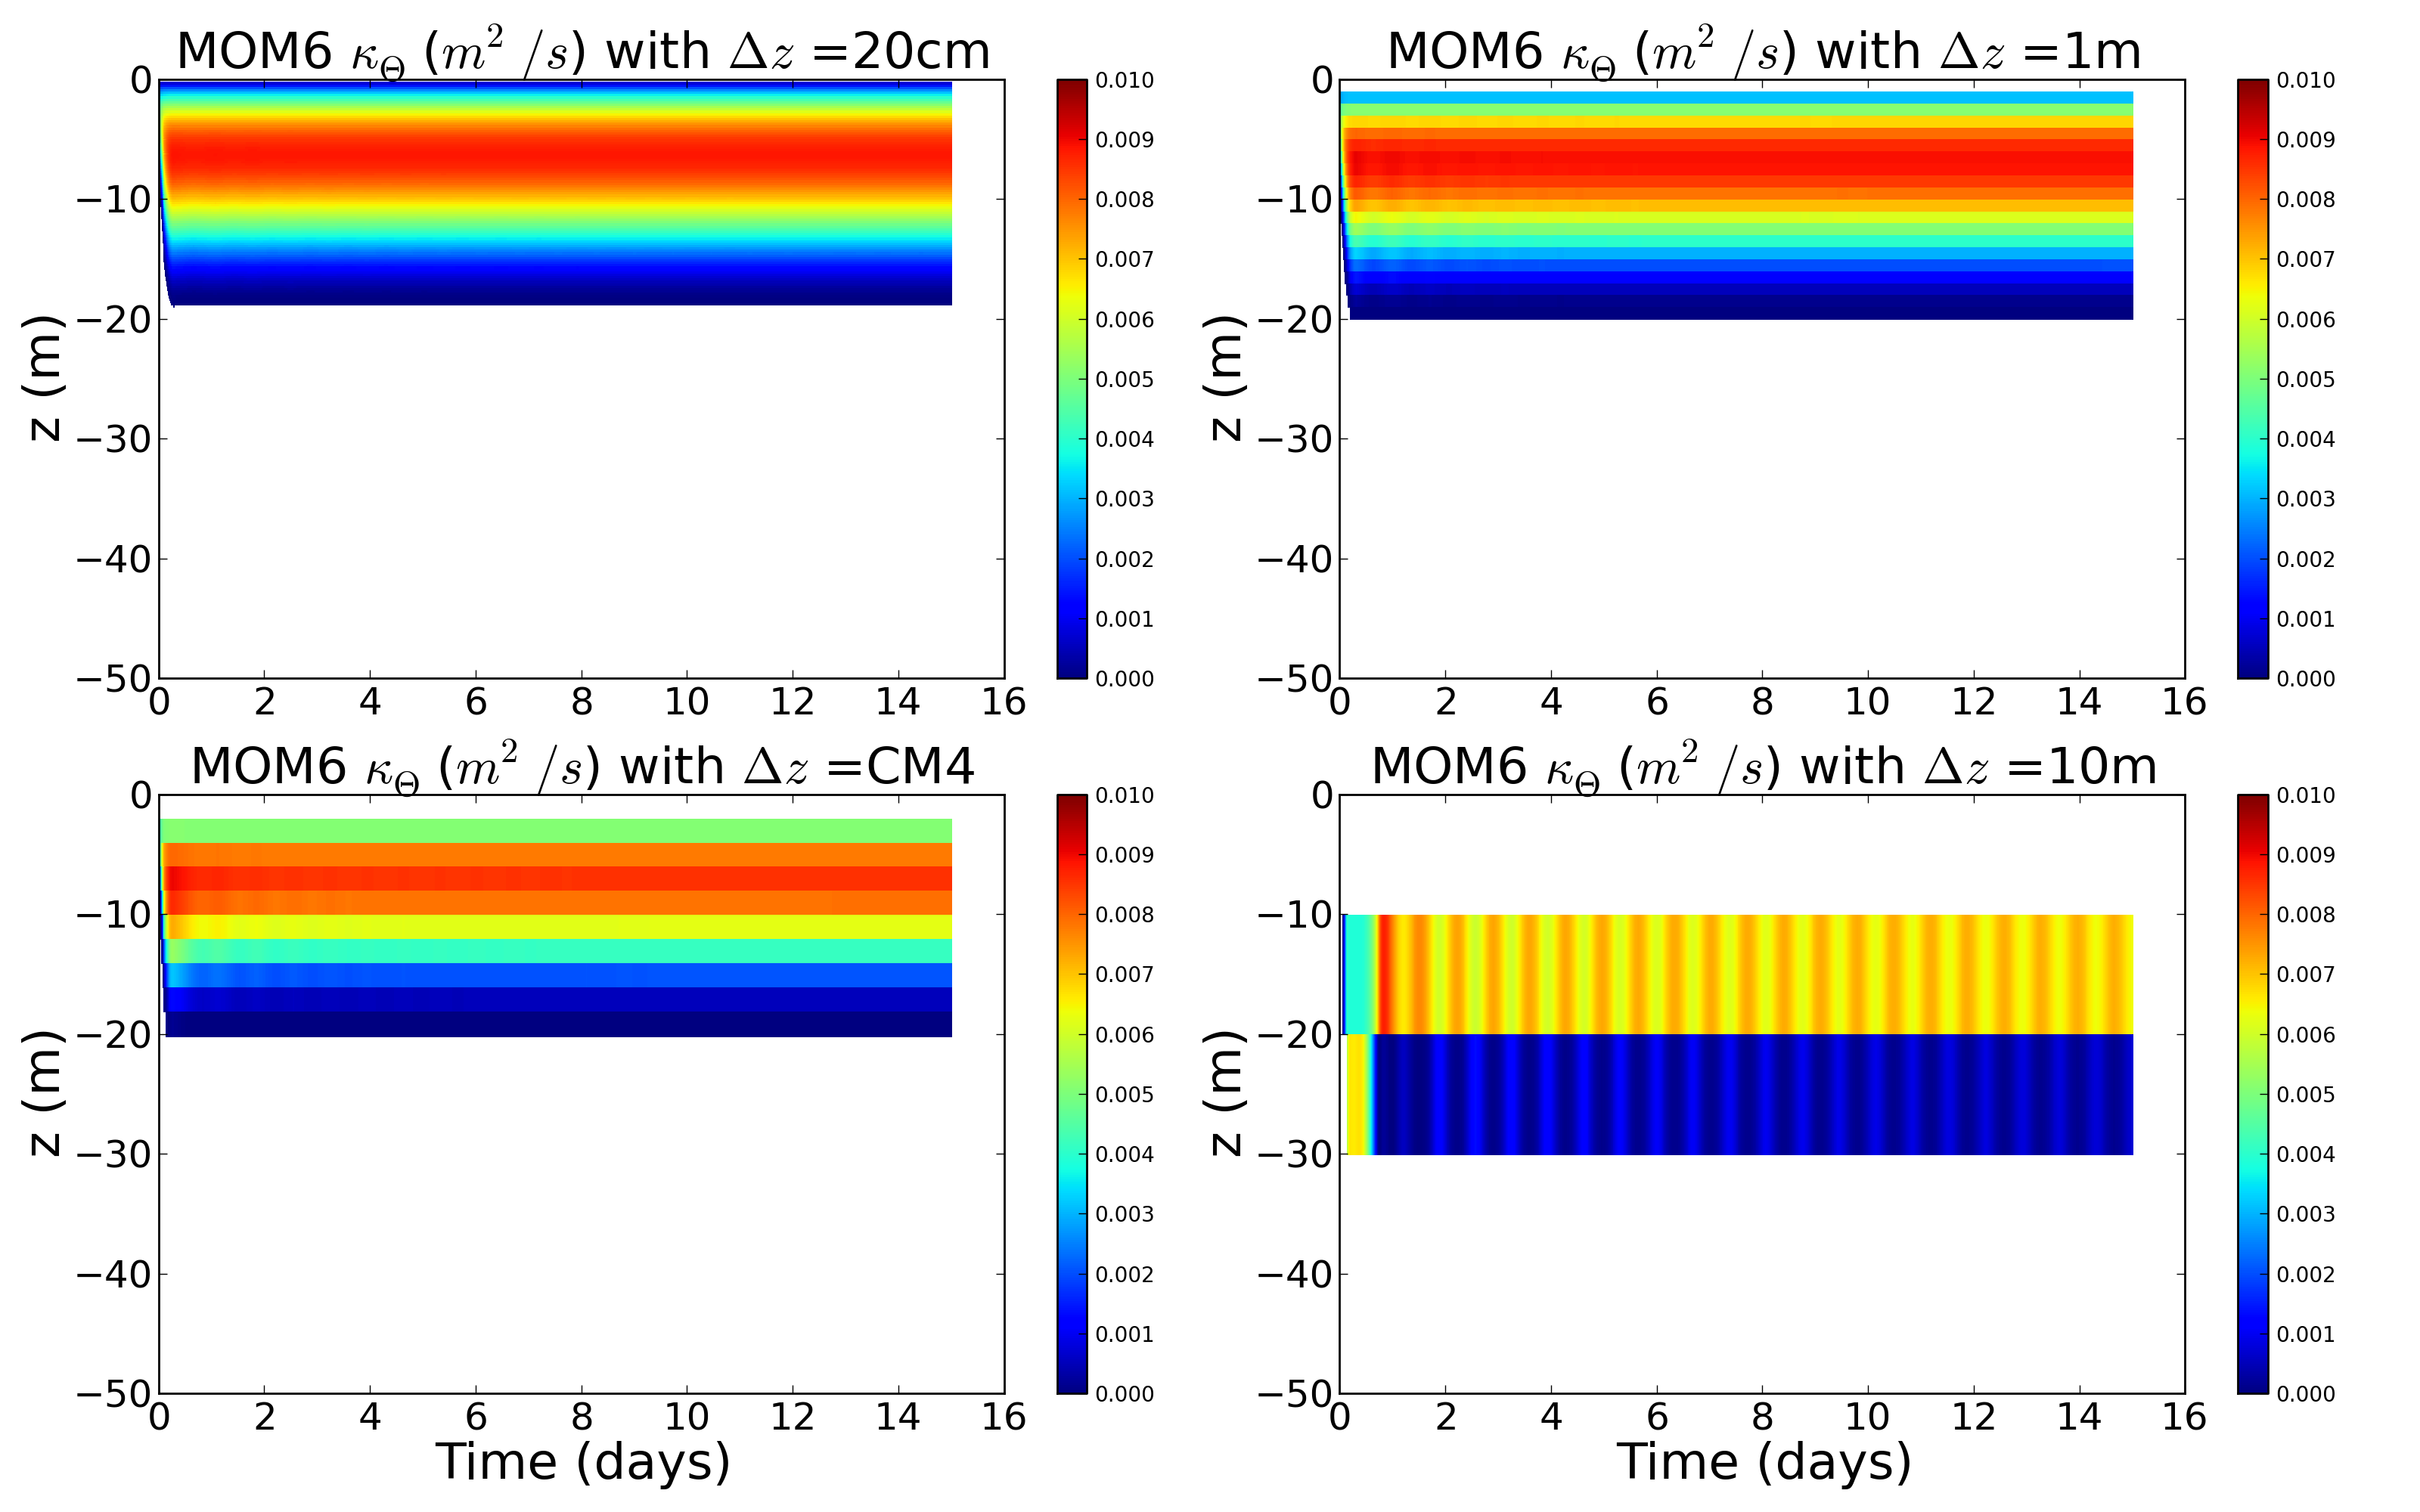
\includegraphics[angle=0,width=14cm]{./figs/MOM6/WSwPSBF_B_MOM6_KPP_diffusivity.png}
\caption[KPP diffusivity from MOM6 for WSwPSBF.B ]{\sf Time series for
  the KPP vertical diffusivity for WSwPSBF.B (constant zonal wind
  stress and $Q=100~\mbox{W}~\mbox{m}^{-2}$) as realized in MOM6 using
  four different vertical grid resolutions.}
\label{fig:WSwPSBF_B_MOM6_KPP_diffusivity}
\end{center}
%\rule{\textwidth}{0.005in}
\end{figure}
%%%%%%%%%%%%%%%%%%%%%%%%%%%%%%%%%%%%%%%%%%%%%%%%%%%%%%%%%%%%%%%%%%%%%%%%


%%%%%%%%%%%%%%%%%%%% %%%%%%%%%%%%%%%%%%%%%%%%%
\begin{figure}[h!t]
%\rule{\textwidth}{0.005in}
\begin{center}
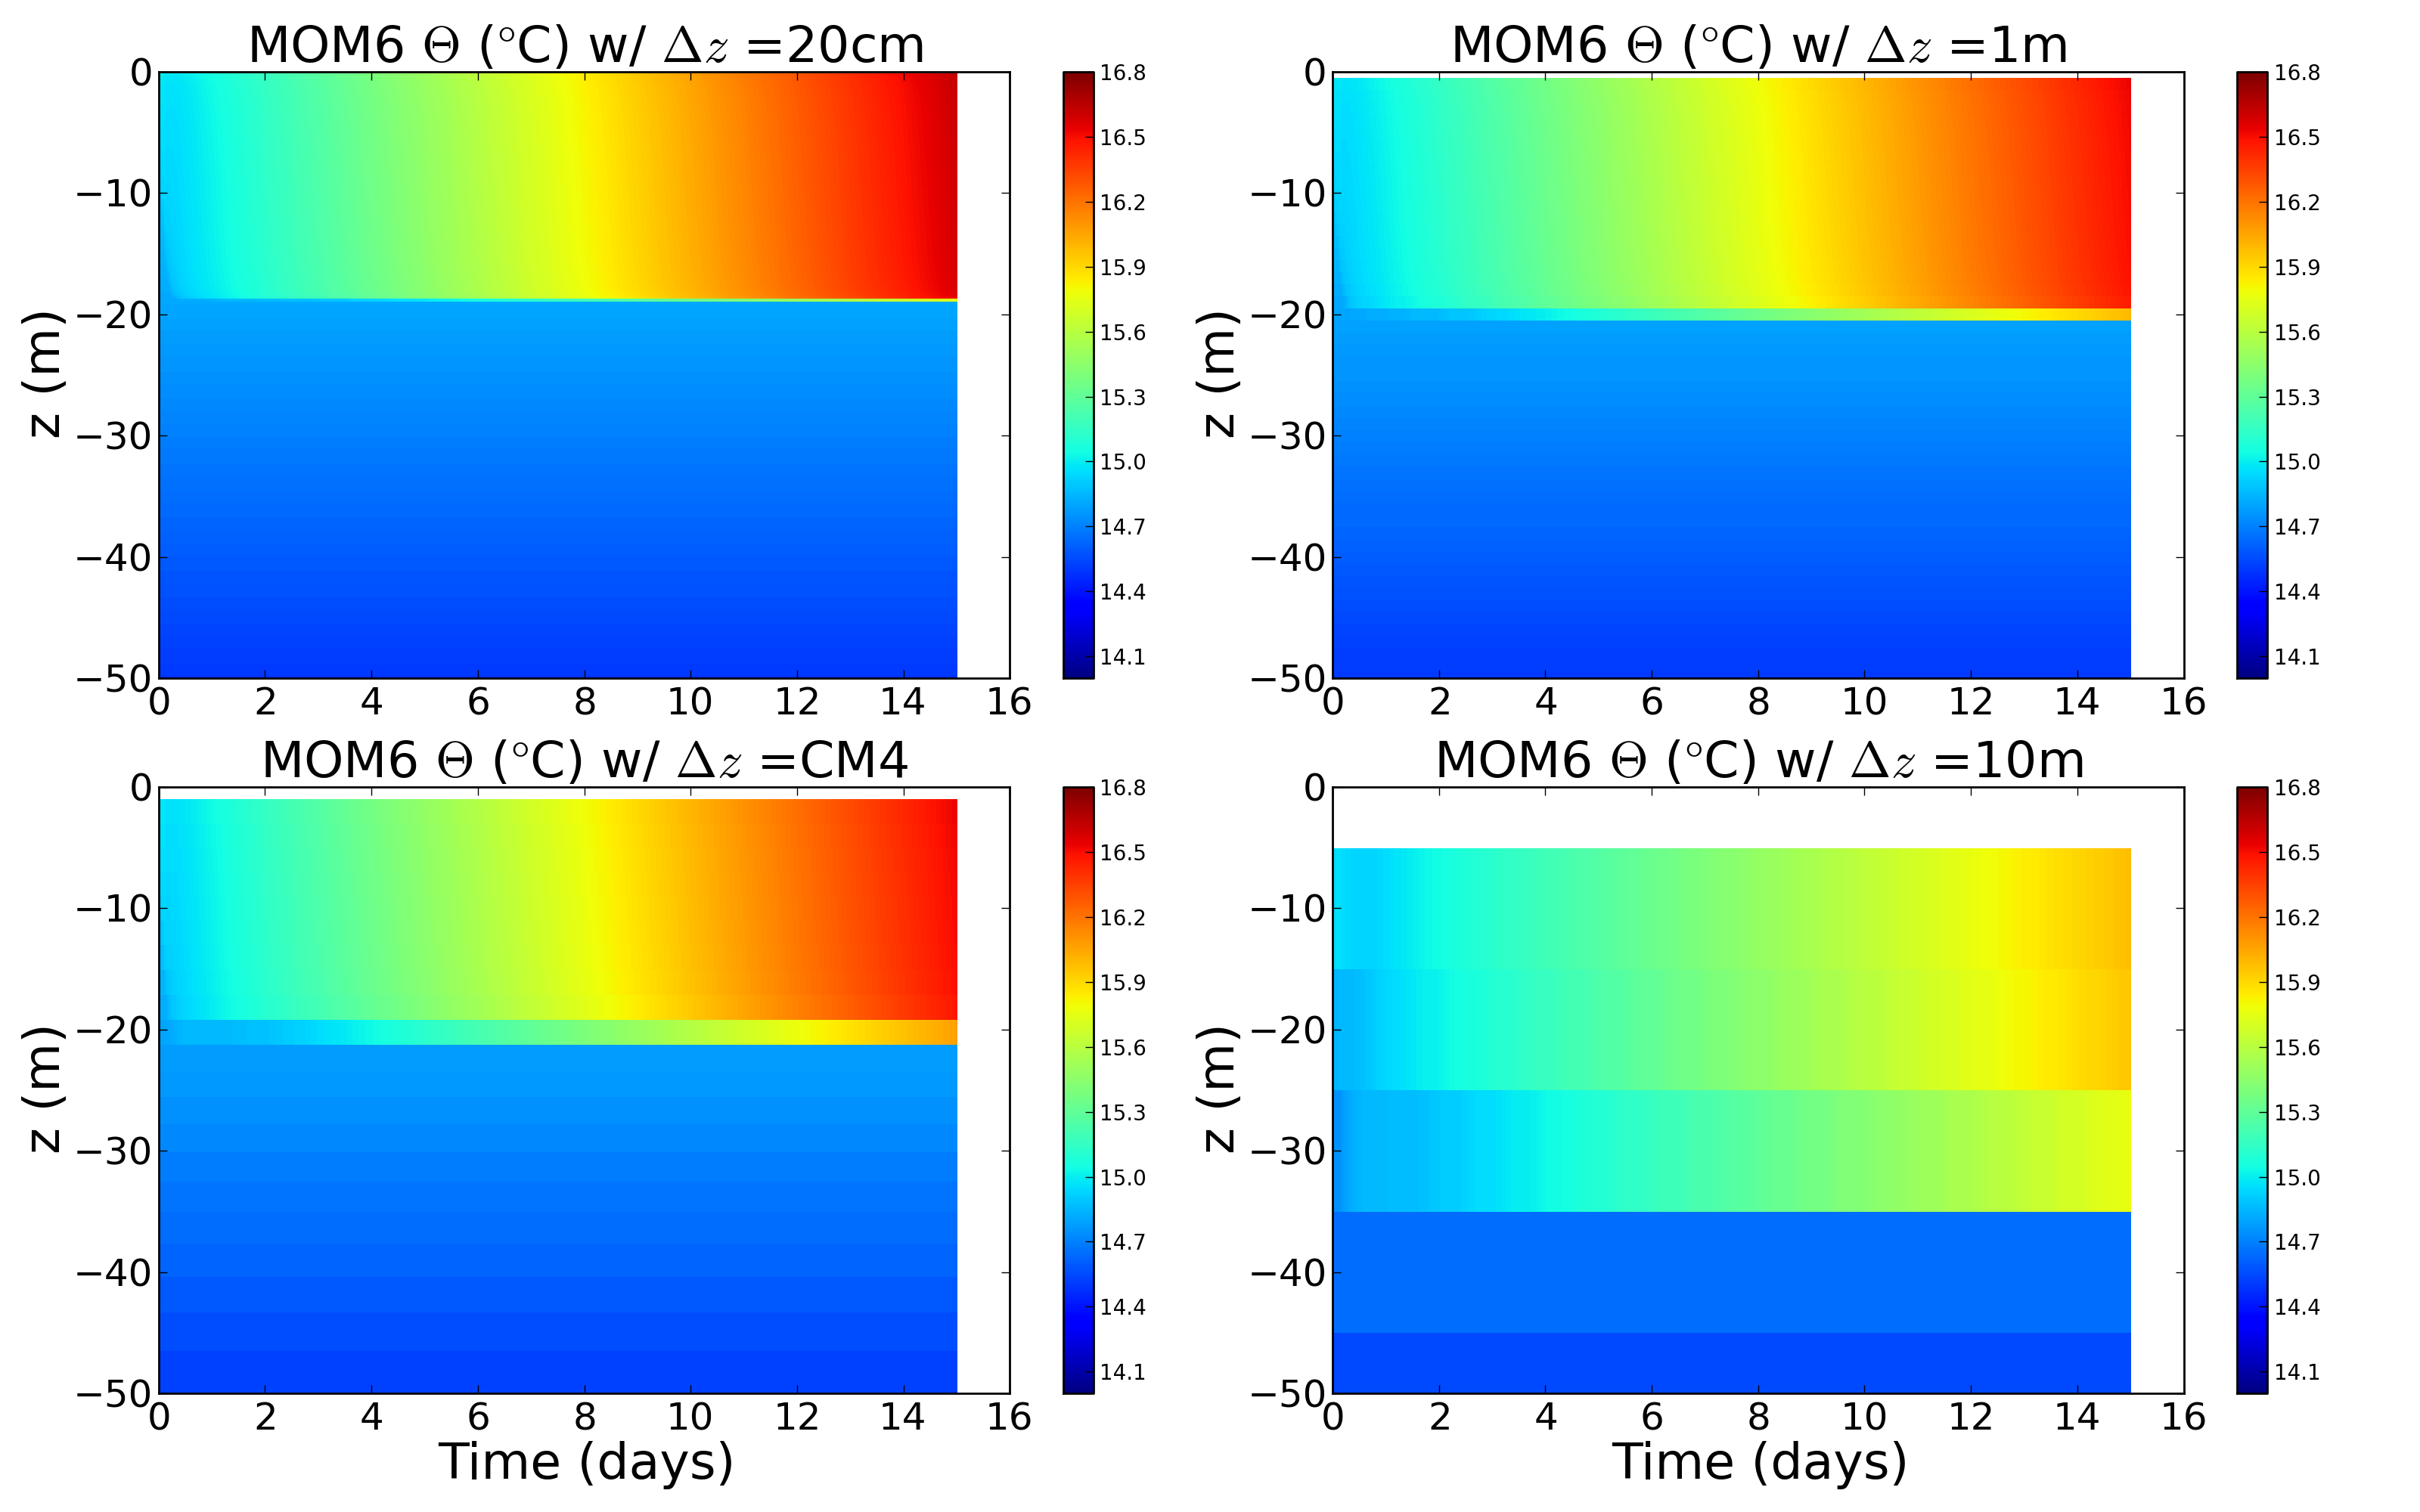
\includegraphics[angle=0,width=14cm]{./figs/MOM6/WSwPSBF_B_MOM6_temp.png}
\caption[Temperature from MOM6 for WSwPSBF.B ]{\sf Time series for
  temperature from test case WSwPSBF.B (constant zonal wind stress and
  $Q=100~\mbox{W}~\mbox{m}^{-2}$) as realized in MOM6 using four
  different vertical grid resolutions.}
\label{fig:WSwPSBF_B_MOM6_temp}
\end{center}
%\rule{\textwidth}{0.005in}
\end{figure}
%%%%%%%%%%%%%%%%%%%%%%%%%%%%%%%%%%%%%%%%%%%%%%%%%%%%%%%%%%%%%%%%%%%%%%%%

%%%%%%%%%%%%%%%%%%%% %%%%%%%%%%%%%%%%%%%%%%%%%
\begin{figure}[h!t]
%\rule{\textwidth}{0.005in}
\begin{center}
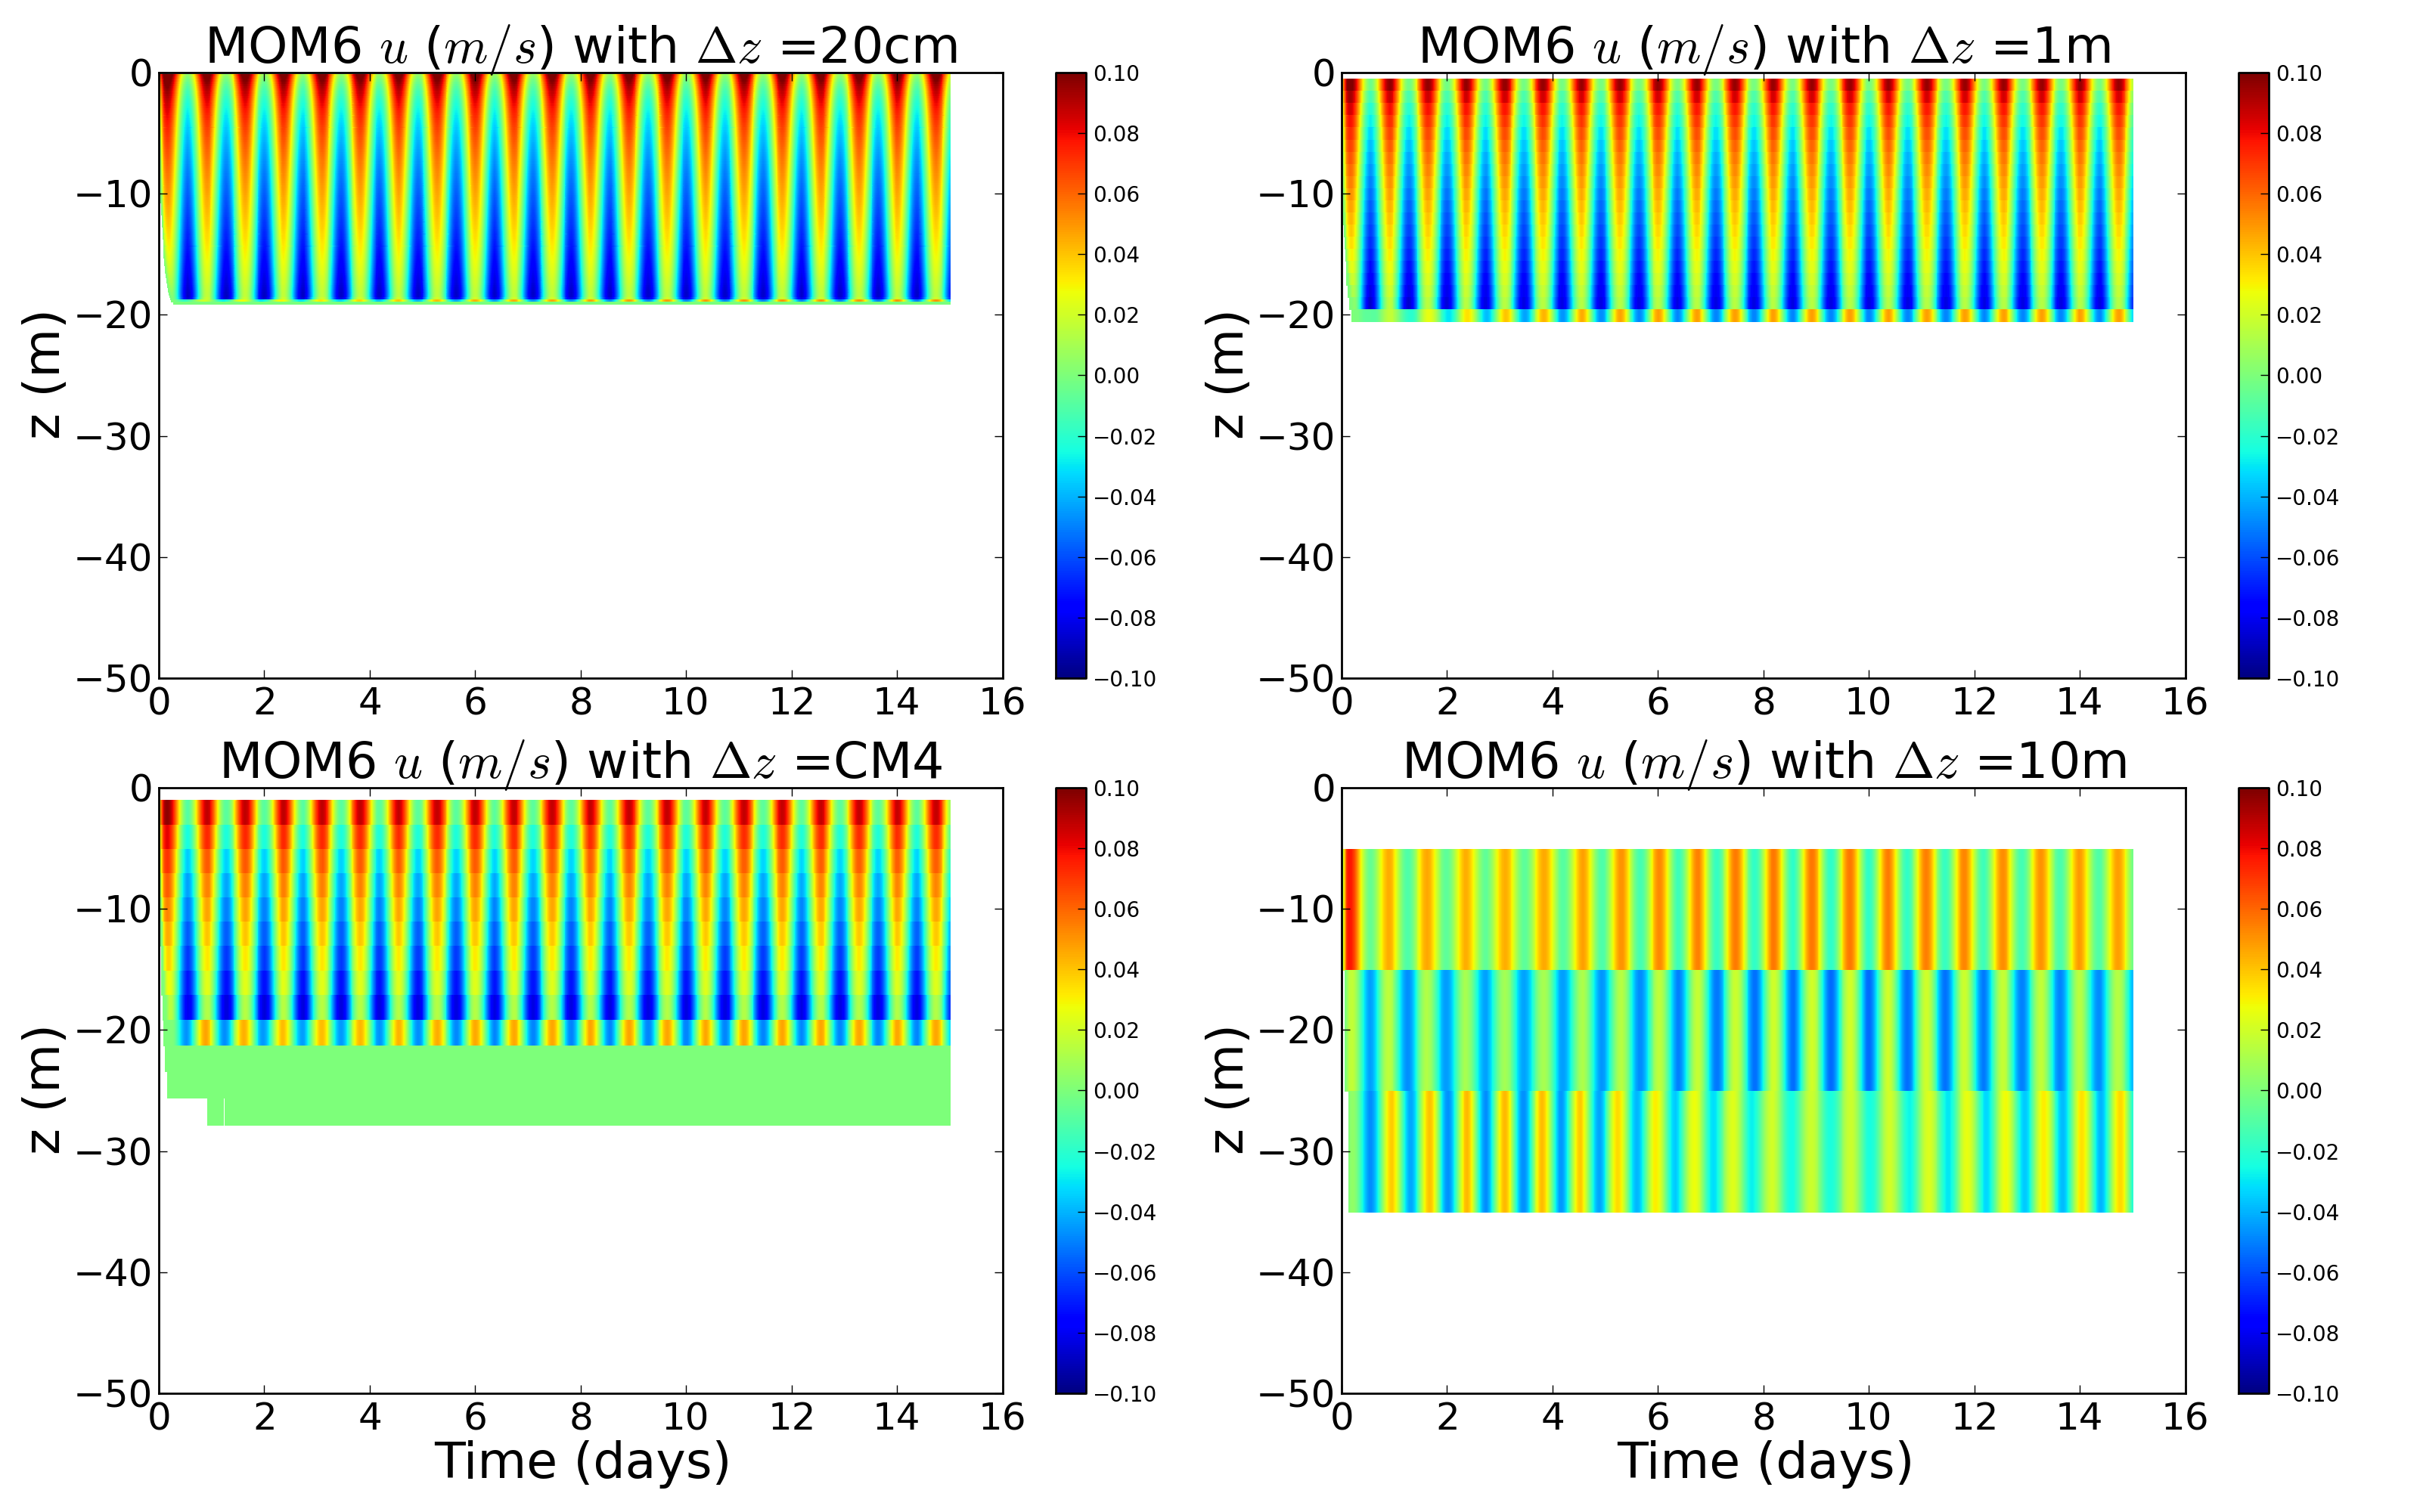
\includegraphics[angle=0,width=14cm]{./figs/MOM6/WSwPSBF_B_MOM6_zonal_velocity.png}
\caption[Zonal velocity from MOM6 for WSwPSBF.B ]{\sf Time series for
  zonal velocity from test case WSwPSBF.B (constant zonal wind stress
  and $Q=100~\mbox{W}~\mbox{m}^{-2}$) as realized in MOM6 using four
  different vertical grid resolutions.}
\label{fig:WSwPSBF_B_MOM6_zonal}
\end{center}
%\rule{\textwidth}{0.005in}
\end{figure}
%%%%%%%%%%%%%%%%%%%%%%%%%%%%%%%%%%%%%%%%%%%%%%%%%%%%%%%%%%%%%%%%%%%%%%%%

\clearpage 




\section{Results for WSwPSBF.C ($Q$ from surface restoring)}
\label{section:WSwPSBFC}

We here present results from the three ocean models for the experiment
WSwPSBF.C, in which there is a restoring surface heat flux as detailed
in equation (\ref{eq:heat-flux-restoring}), along with the constant
zonal wind stress $\tau^{x} = 0.1~\mbox{N}~\mbox{m}^{-2}$.  Given that
the surface restoring is to a temperature warmer than the initial SST,
the buoyancy forcing is positive.  The results for this test are very
similar to test WSwPSBF.B.  In particular, results here illustrate the
problems with the coarsest grid resolution $\Delta z = 10~\mbox{m}$.

\subsection{GFDL-MOM6} 

Figure \ref{fig:WSwPSBF_C_MOM6_SST_bldepth} shows the KPP boundary
layer depth from the MOM6 implementation of CVMix.  The boundary layer
rapidly deepens to roughly $14~\mbox{m}$, and then remains nearly for
most of the 15 day simulation.  There is a notable oscillation of the
boundary layer depth in the coarsest resolution with $\Delta z =
10~\mbox{m}$, whereas the other grids show relatively steady values by
roughly three days.  The oscillations have a period shorter than the
inertial period of roughly $0.73~\mbox{days}$ (equation
(\ref{eq:inertial-period})).  The SST steadily rises from the positive
surface heat flux, which dominates over the effects of wind mixing.
The surface heat flux reduces in time as the SST approaches the
restoring value $\Theta_{\mbox{\footnotesize restore}} = \Theta_s +
10^{\circ}C$ (equation (\ref{eq:restoring-temp})), where $\Theta_s =
15.0^{\circ}C$ (equation (\ref{eq:thetas})). 

The SST is cooler as the grid coarsens, with the coarsest grid $\Delta
z = 10~\mbox{m}$ most notably cooler.  The reason is that as the
vertical grid spacing increases, the first non-zero KPP diffusivity
occurs at the bottom interface of the surface cell, which reaches
deeper into the cooler interior as the grid coarsens (see Figure
\ref{fig:WSwPSBF_C_MOM6_KPP_diffusivity}).  Particularly with $\Delta
z = 10~\mbox{m}$, we see how the bottom of the top cell reaches into
the cooler interior more than the finer grids, and thus brings the
surface cell into contact with relatively cool interior waters.
Additionally, note how the KPP diffusivity with $\Delta z =
10~\mbox{m}$ exhibits an oscillatory behaviour, reflecting the
inertial oscillations in the boundary layer depth for this resolution.
Figure \ref{fig:WSwPSBF_C_MOM6_temp} shows impacts of the upper ocean
heating on the depth profile of temperature, Figure
\ref{fig:WSwPSBF_C_MOM6_zonal} exhibits inertial oscillations in zonal
velocity associated with the zonal wind stress.

%%%%%%%%%%%%%%%%%%%% %%%%%%%%%%%%%%%%%%%%%%%%%
\begin{figure}[h!t]
%\rule{\textwidth}{0.005in}
\begin{center}
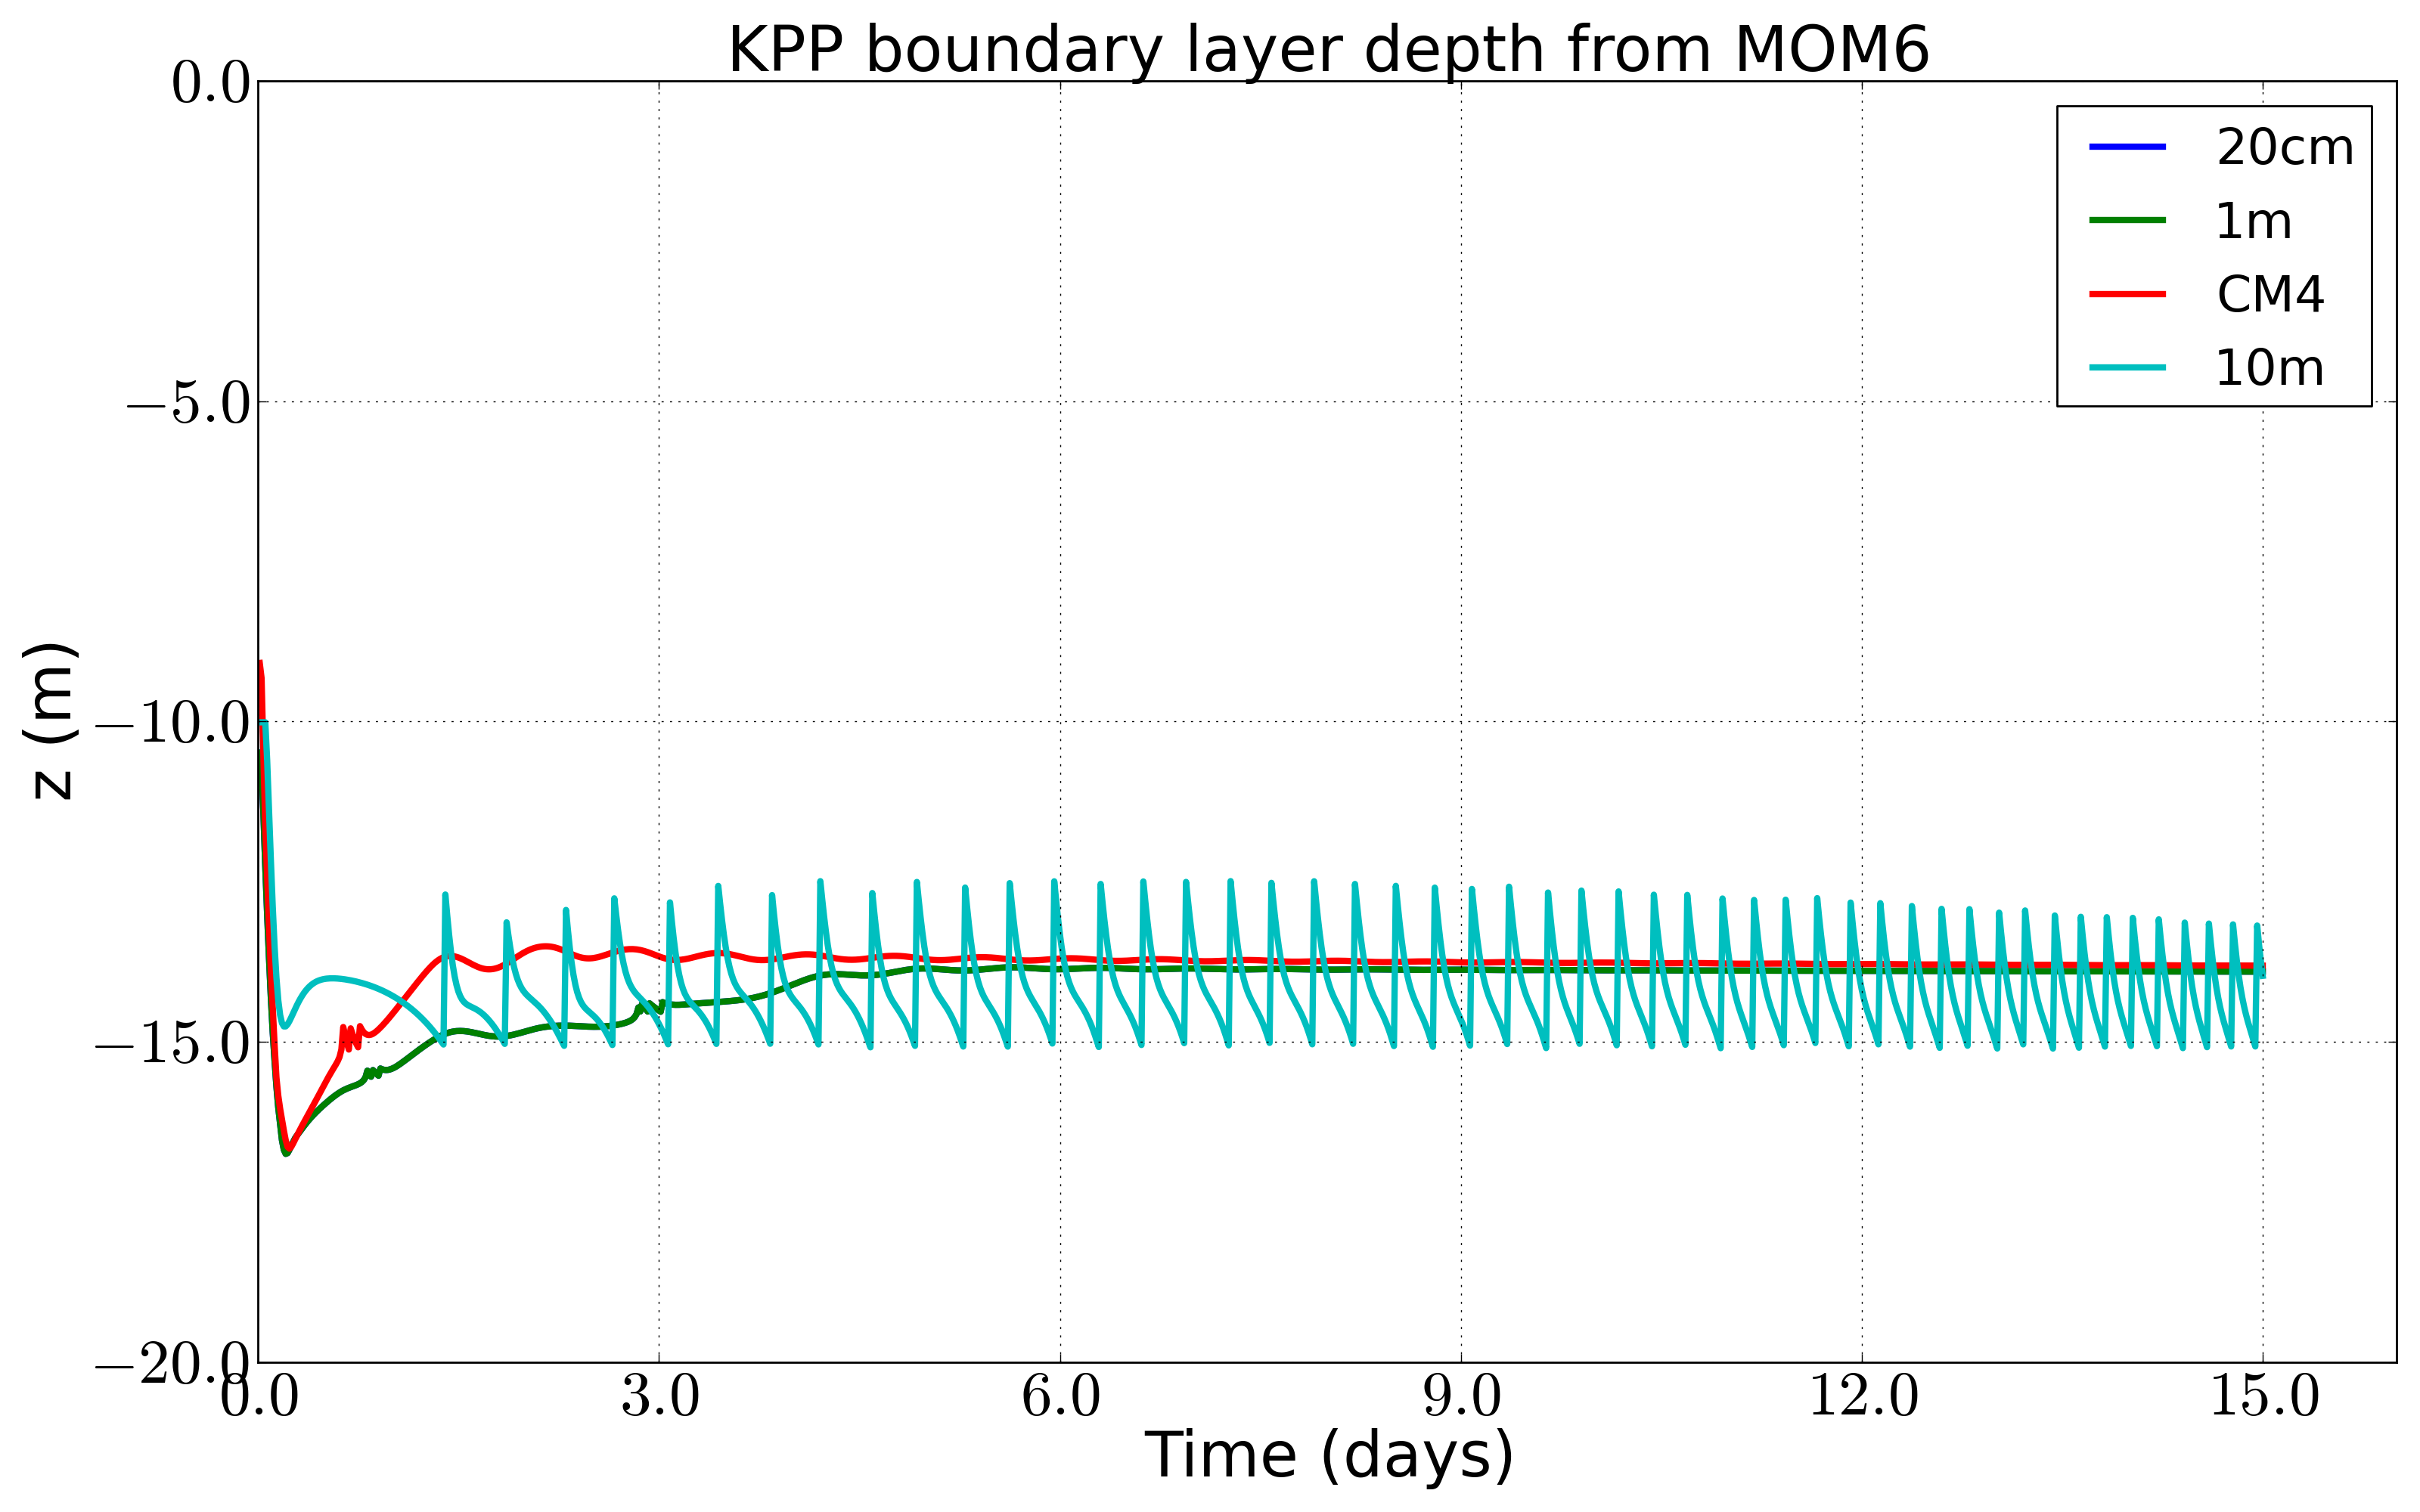
\includegraphics[angle=0,width=8cm]{./figs/MOM6/WSwPSBF_C_MOM6_KPP_bldepth.png}
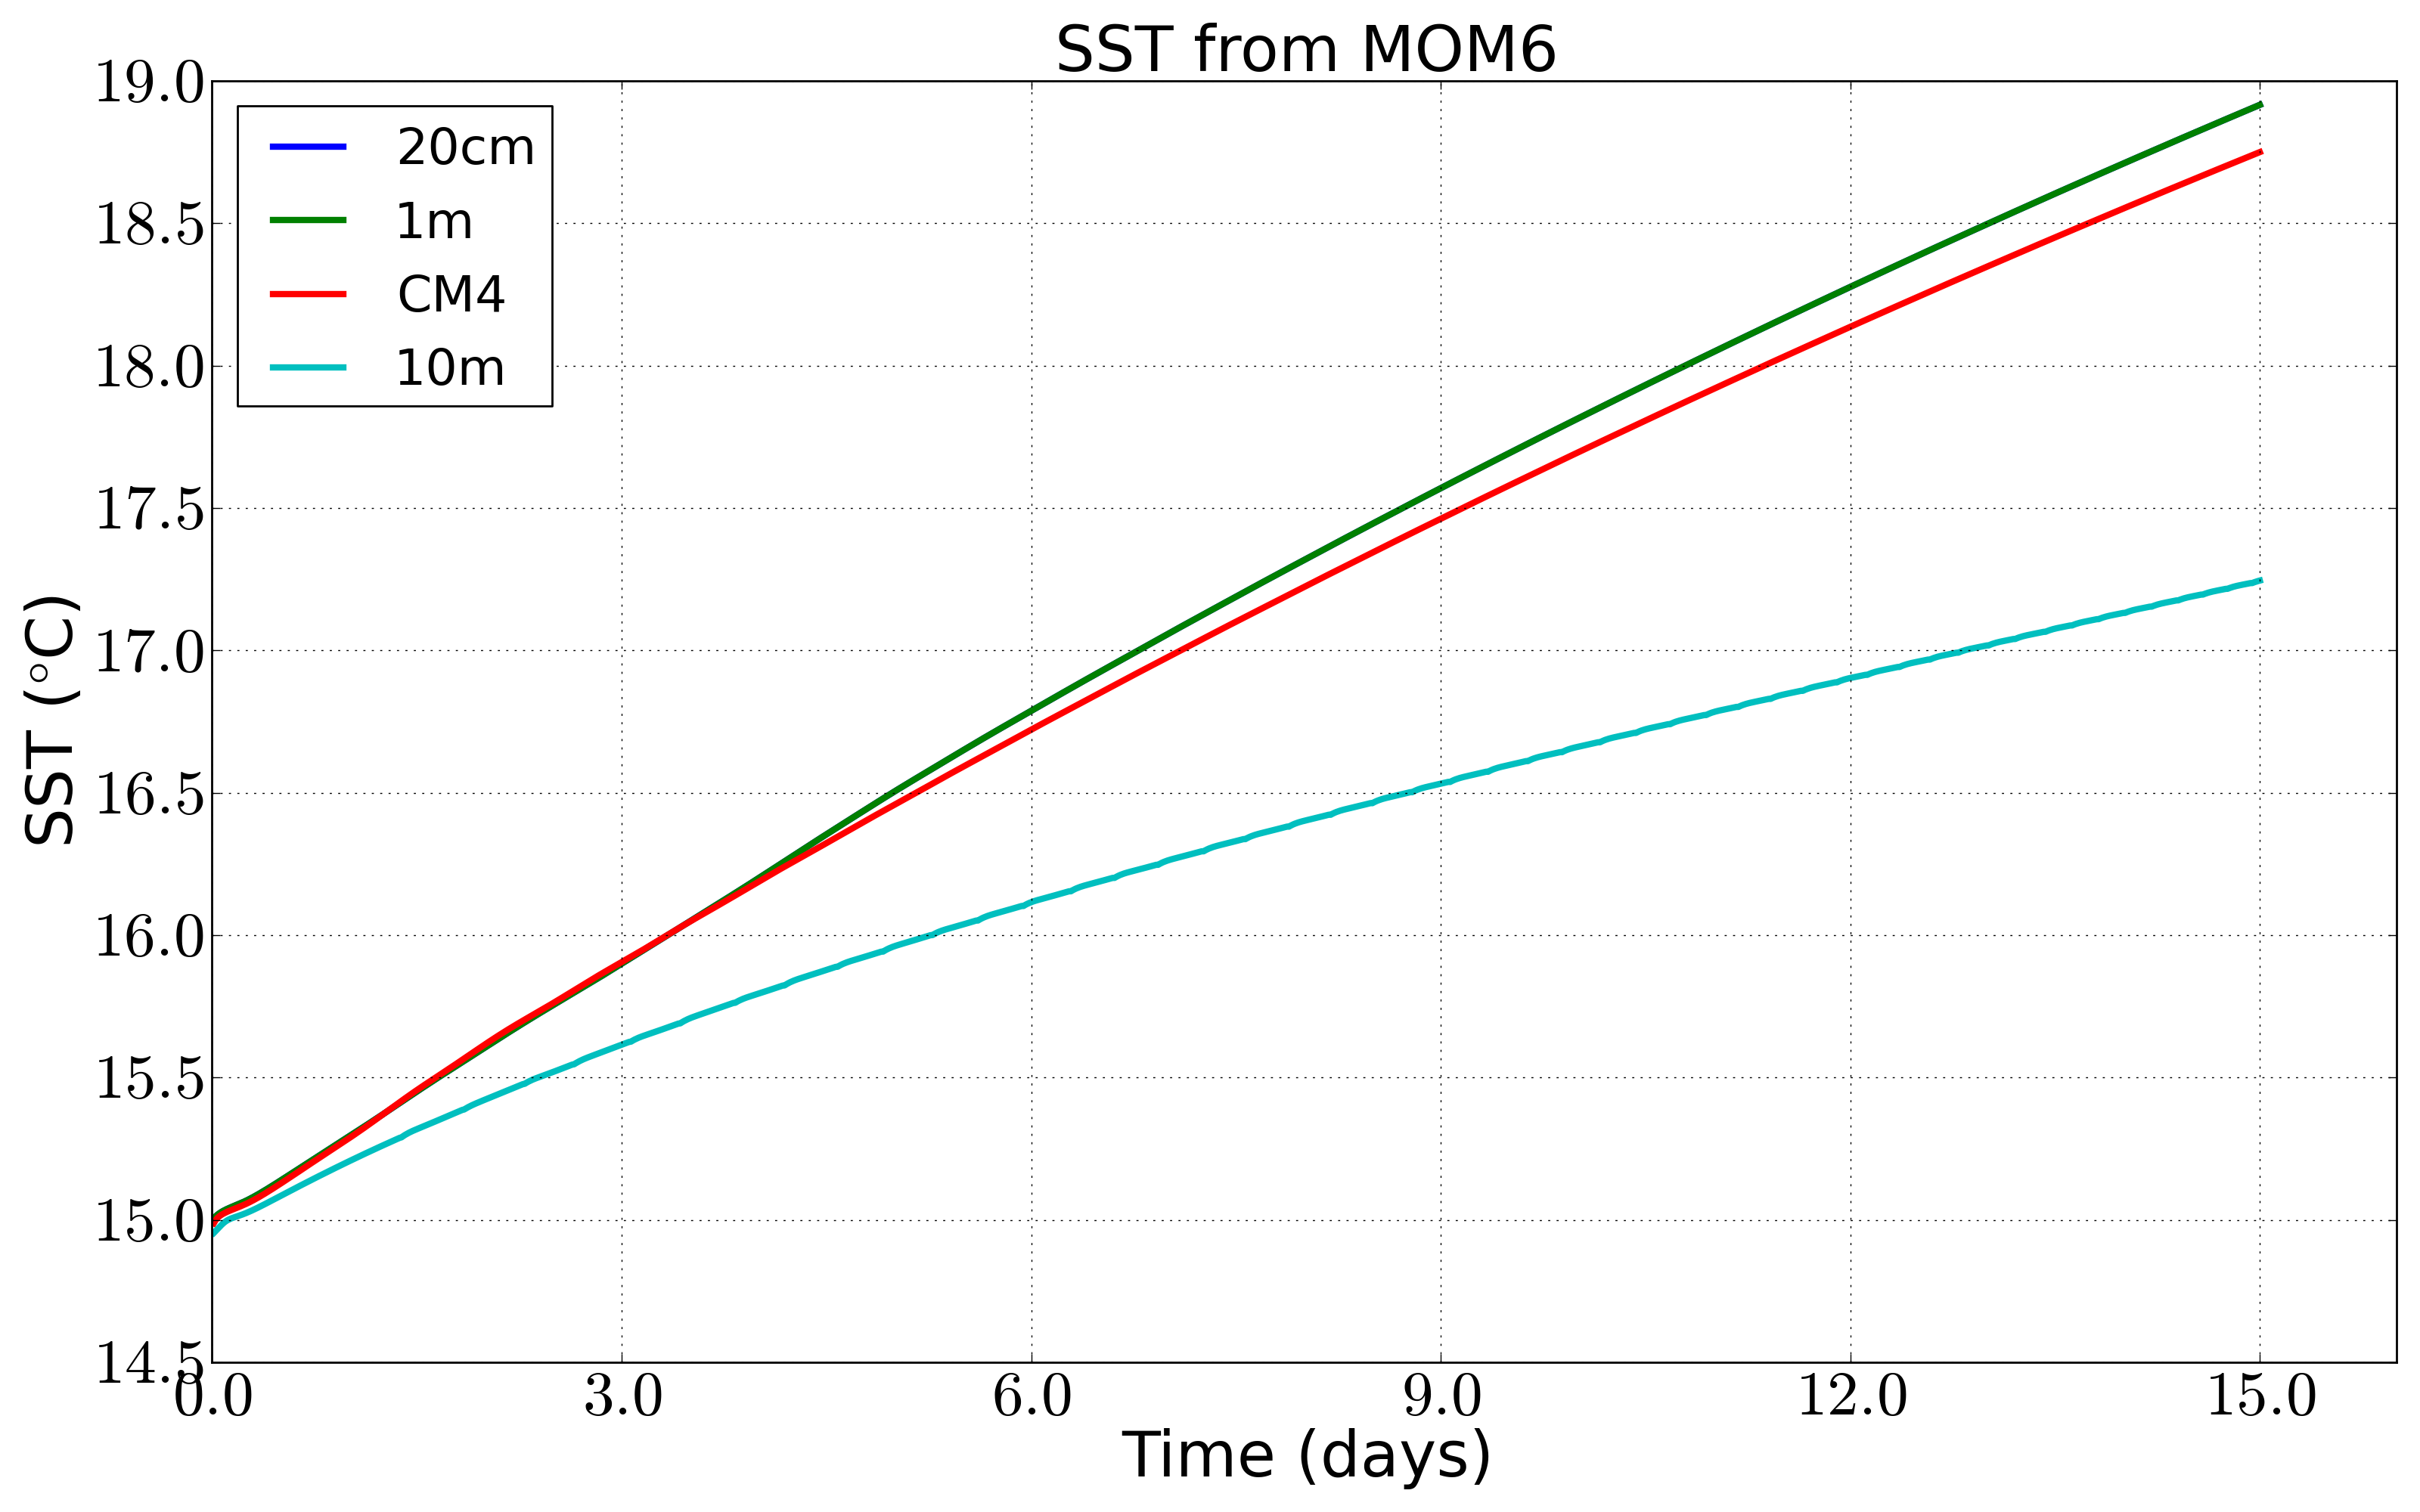
\includegraphics[angle=0,width=8cm]{./figs/MOM6/WSwPSBF_C_MOM6_SST.png}
\caption[KPP boundary layer depth and SST from MOM6 for WSwPSBF.C]
{\sf Time series for KPP boundary layer depth (left panel) and SST
  (right panel) for WSwPSBF.C (constant zonal wind stress and
  restoring heat flux) as realized in MOM6.}
\label{fig:WSwPSBF_C_MOM6_SST_bldepth}
\end{center}
%\rule{\textwidth}{0.005in}
\end{figure}
%%%%%%%%%%%%%%%%%%%%%%%%%%%%%%%%%%%%%%%%%%%%%%%%%%%%%%%%%%%%%%%%%%%%%%%%


%%%%%%%%%%%%%%%%%%%% %%%%%%%%%%%%%%%%%%%%%%%%%
\begin{figure}[h!t]
%\rule{\textwidth}{0.005in}
\begin{center}
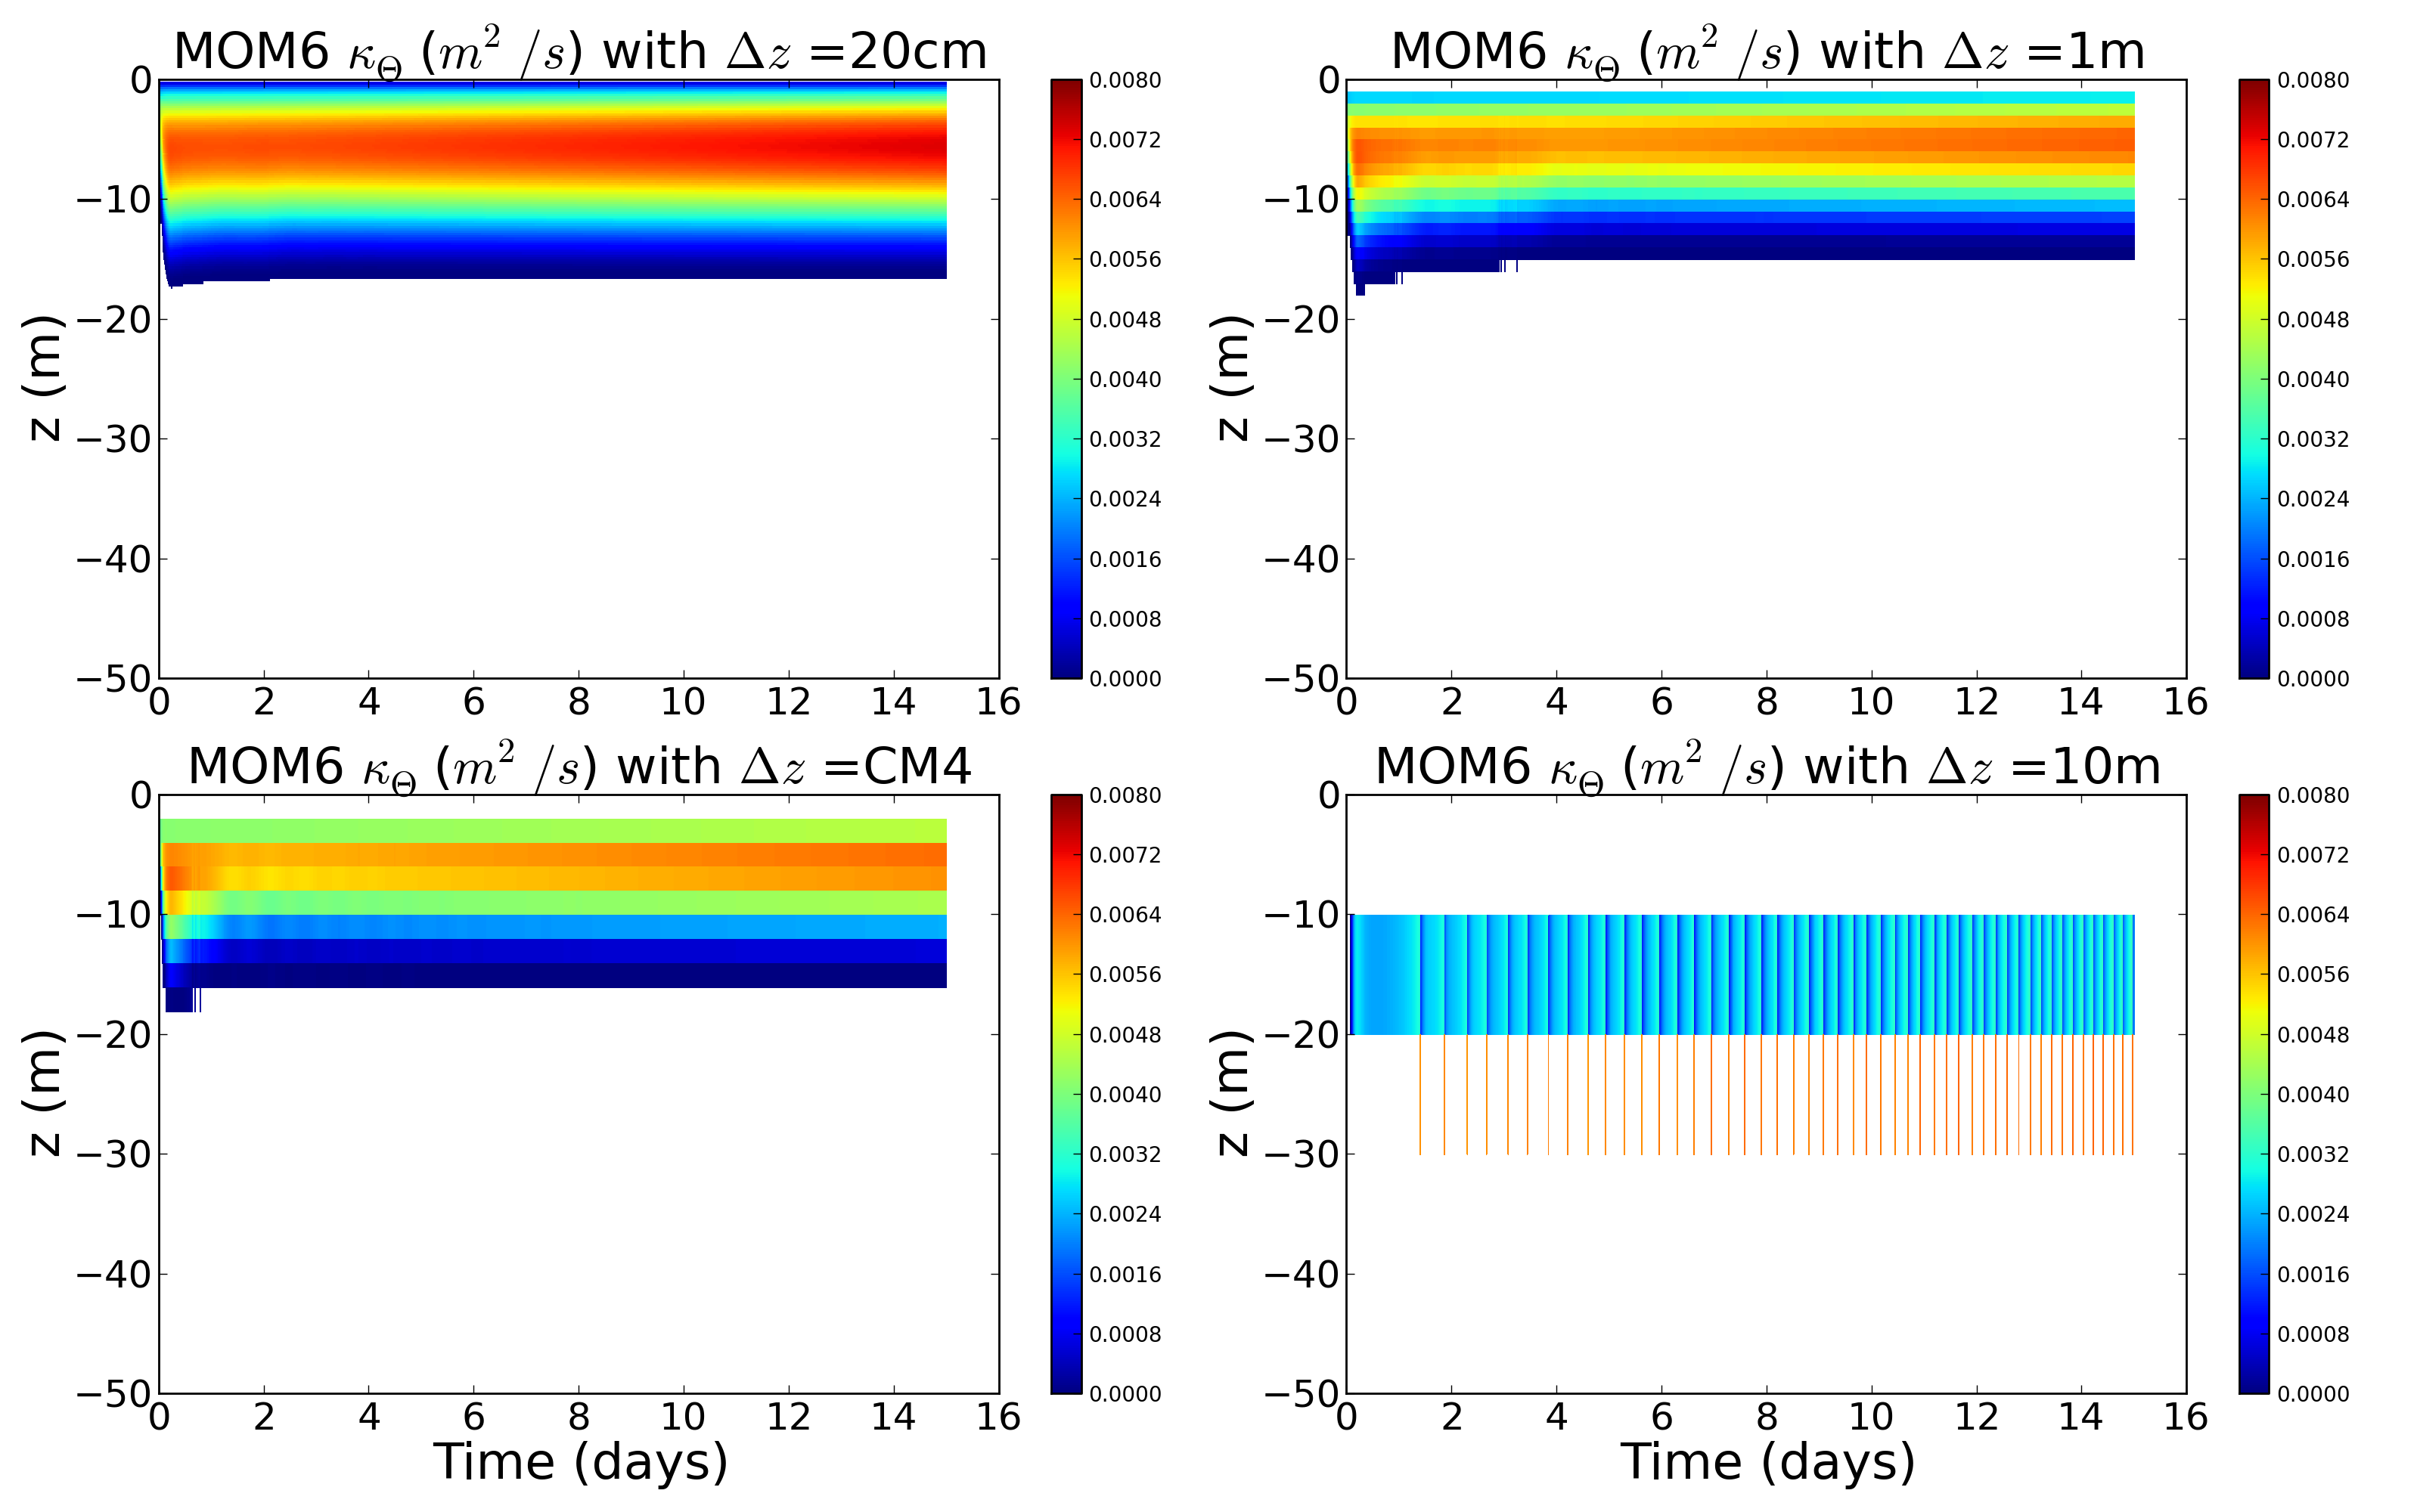
\includegraphics[angle=0,width=14cm]{./figs/MOM6/WSwPSBF_C_MOM6_KPP_diffusivity.png}
\caption[KPP diffusivity from MOM6 for WSwPSBF.C ]{\sf Time series for
  the KPP vertical diffusivity for WSwPSBF.C (constant zonal wind
  stress and restoring heat flux) as realized in MOM6 using four
  different vertical grid resolutions.}
\label{fig:WSwPSBF_C_MOM6_KPP_diffusivity}
\end{center}
%\rule{\textwidth}{0.005in}
\end{figure}
%%%%%%%%%%%%%%%%%%%%%%%%%%%%%%%%%%%%%%%%%%%%%%%%%%%%%%%%%%%%%%%%%%%%%%%%


%%%%%%%%%%%%%%%%%%%% %%%%%%%%%%%%%%%%%%%%%%%%%
\begin{figure}[h!t]
%\rule{\textwidth}{0.005in}
\begin{center}
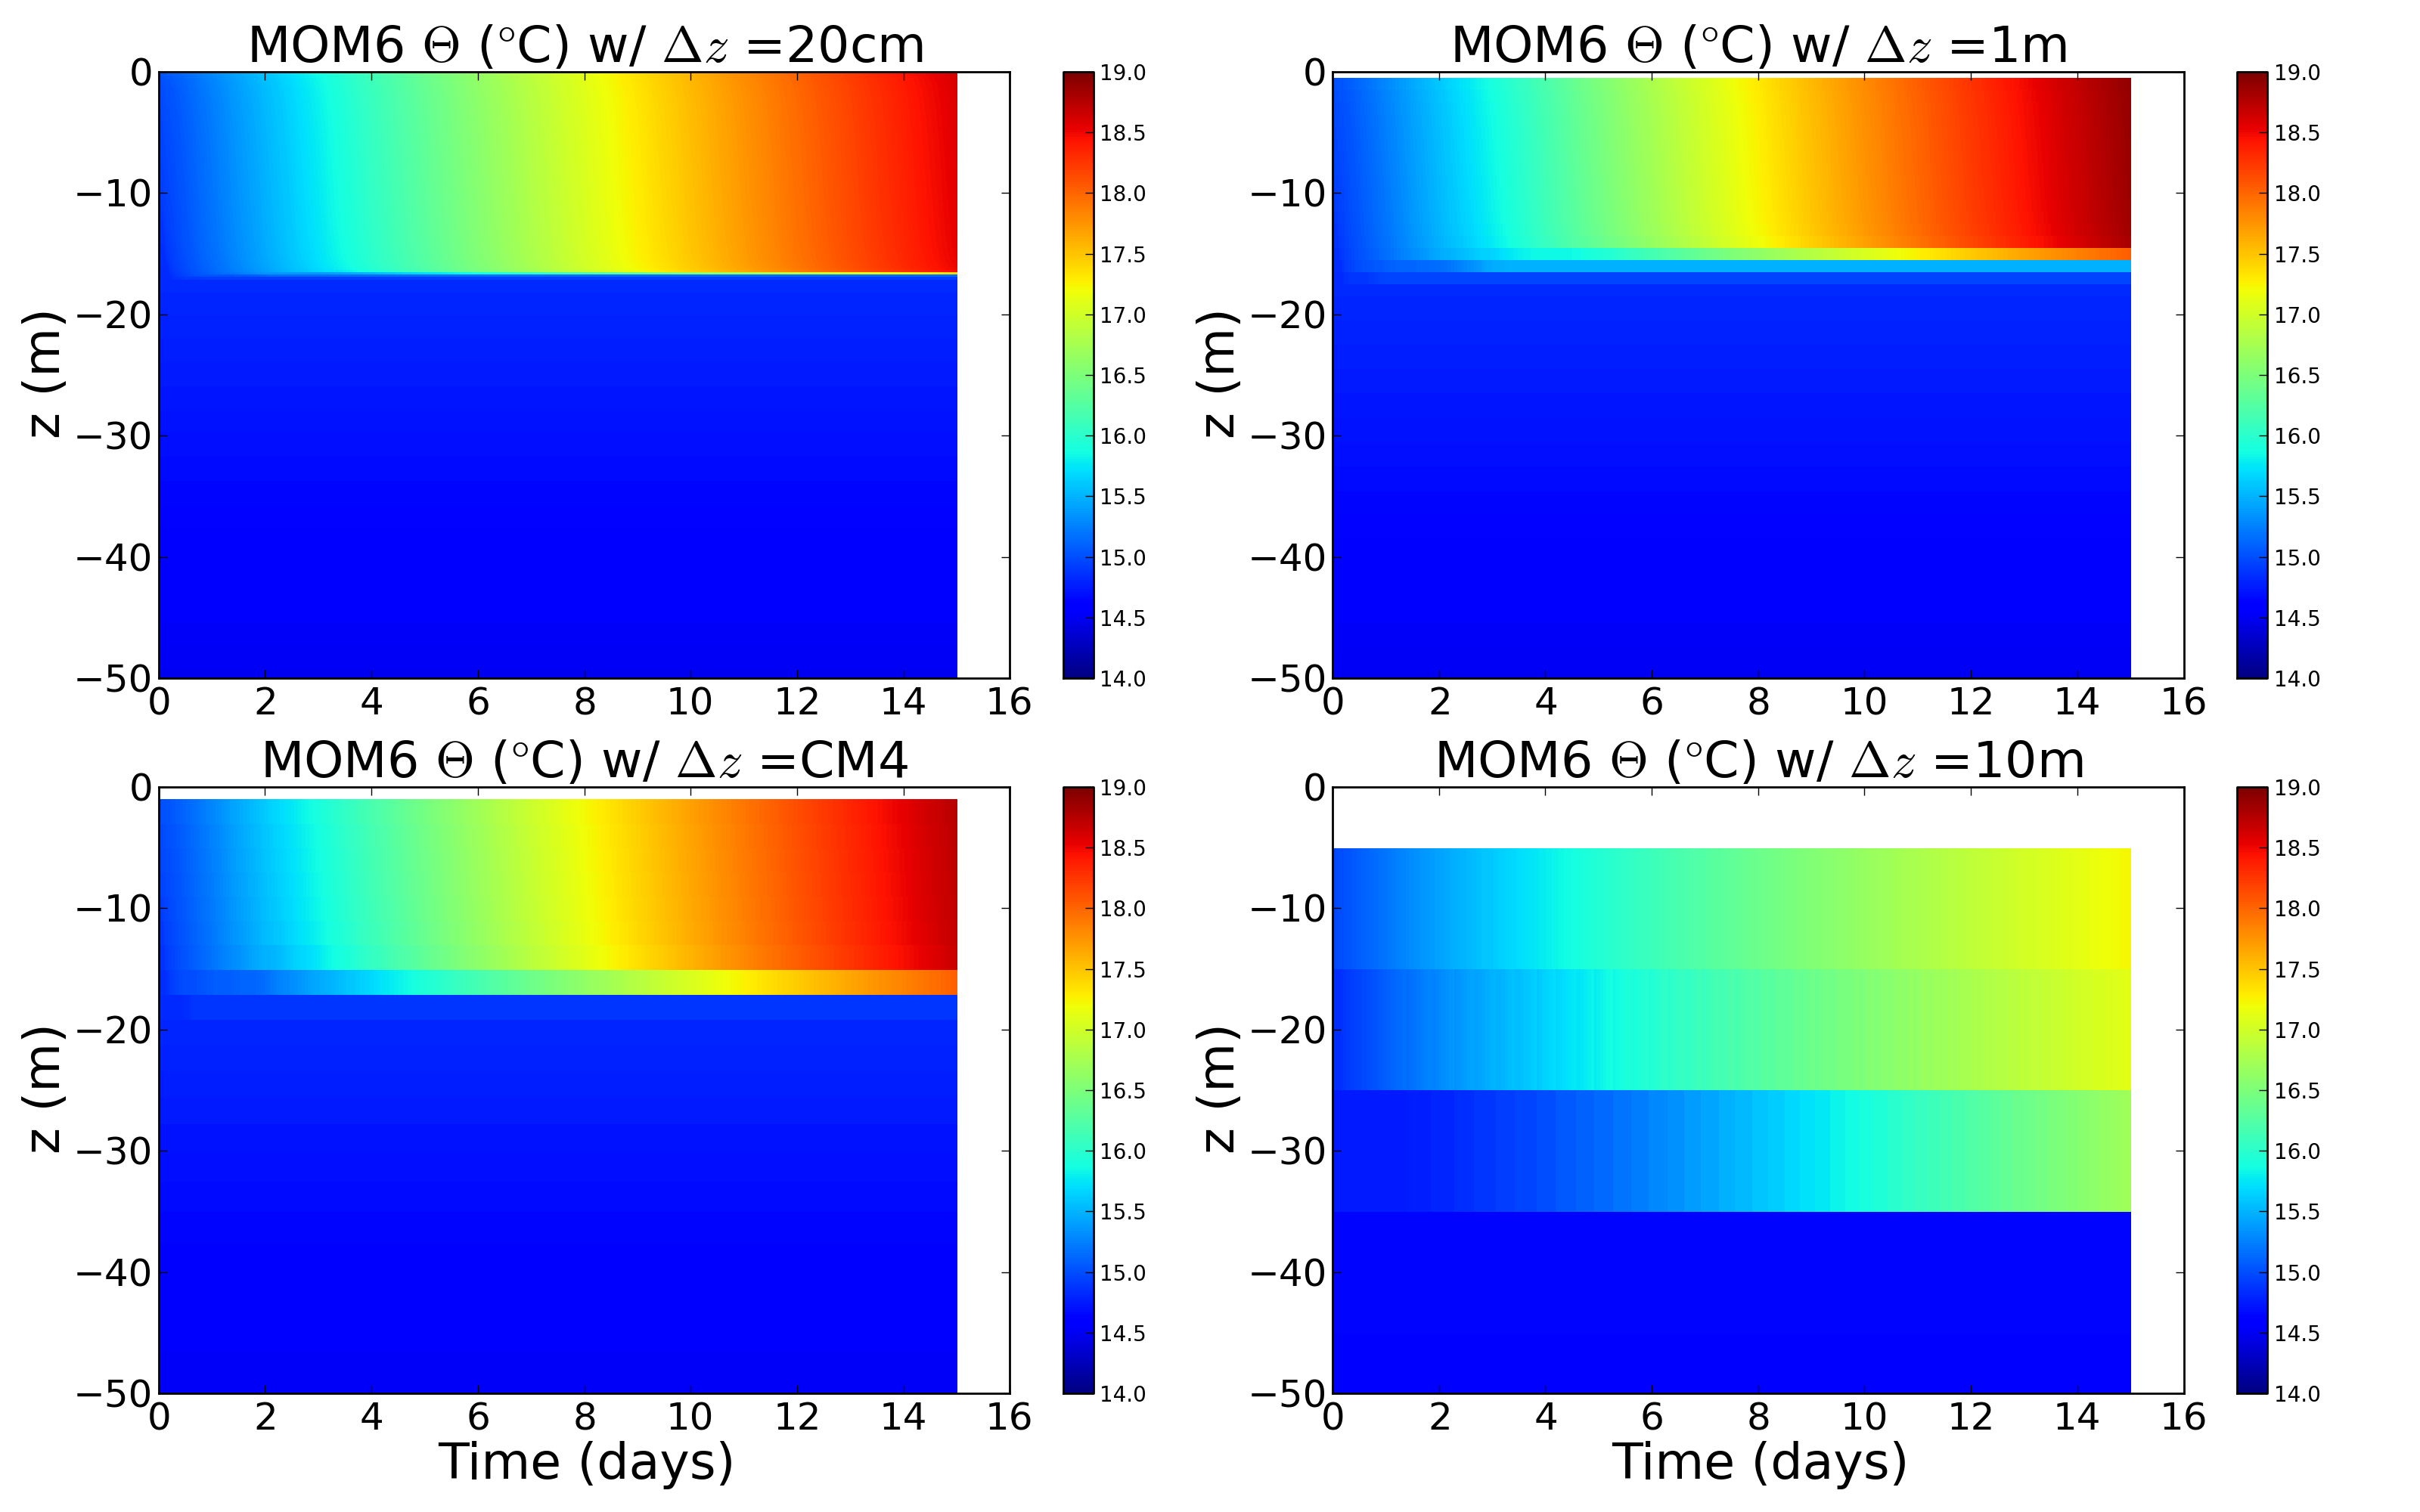
\includegraphics[angle=0,width=14cm]{./figs/MOM6/WSwPSBF_C_MOM6_temp.png}
\caption[Temperature from MOM6 for WSwPSBF.C ]{\sf Time series for
  temperature from test case WSwPSBF.C (constant zonal wind stress and
  restoring heat flux) as realized in MOM6 using four different
  vertical grid resolutions.}
\label{fig:WSwPSBF_C_MOM6_temp}
\end{center}
%\rule{\textwidth}{0.005in}
\end{figure}
%%%%%%%%%%%%%%%%%%%%%%%%%%%%%%%%%%%%%%%%%%%%%%%%%%%%%%%%%%%%%%%%%%%%%%%%

%%%%%%%%%%%%%%%%%%%% %%%%%%%%%%%%%%%%%%%%%%%%%
\begin{figure}[h!t]
%\rule{\textwidth}{0.005in}
\begin{center}
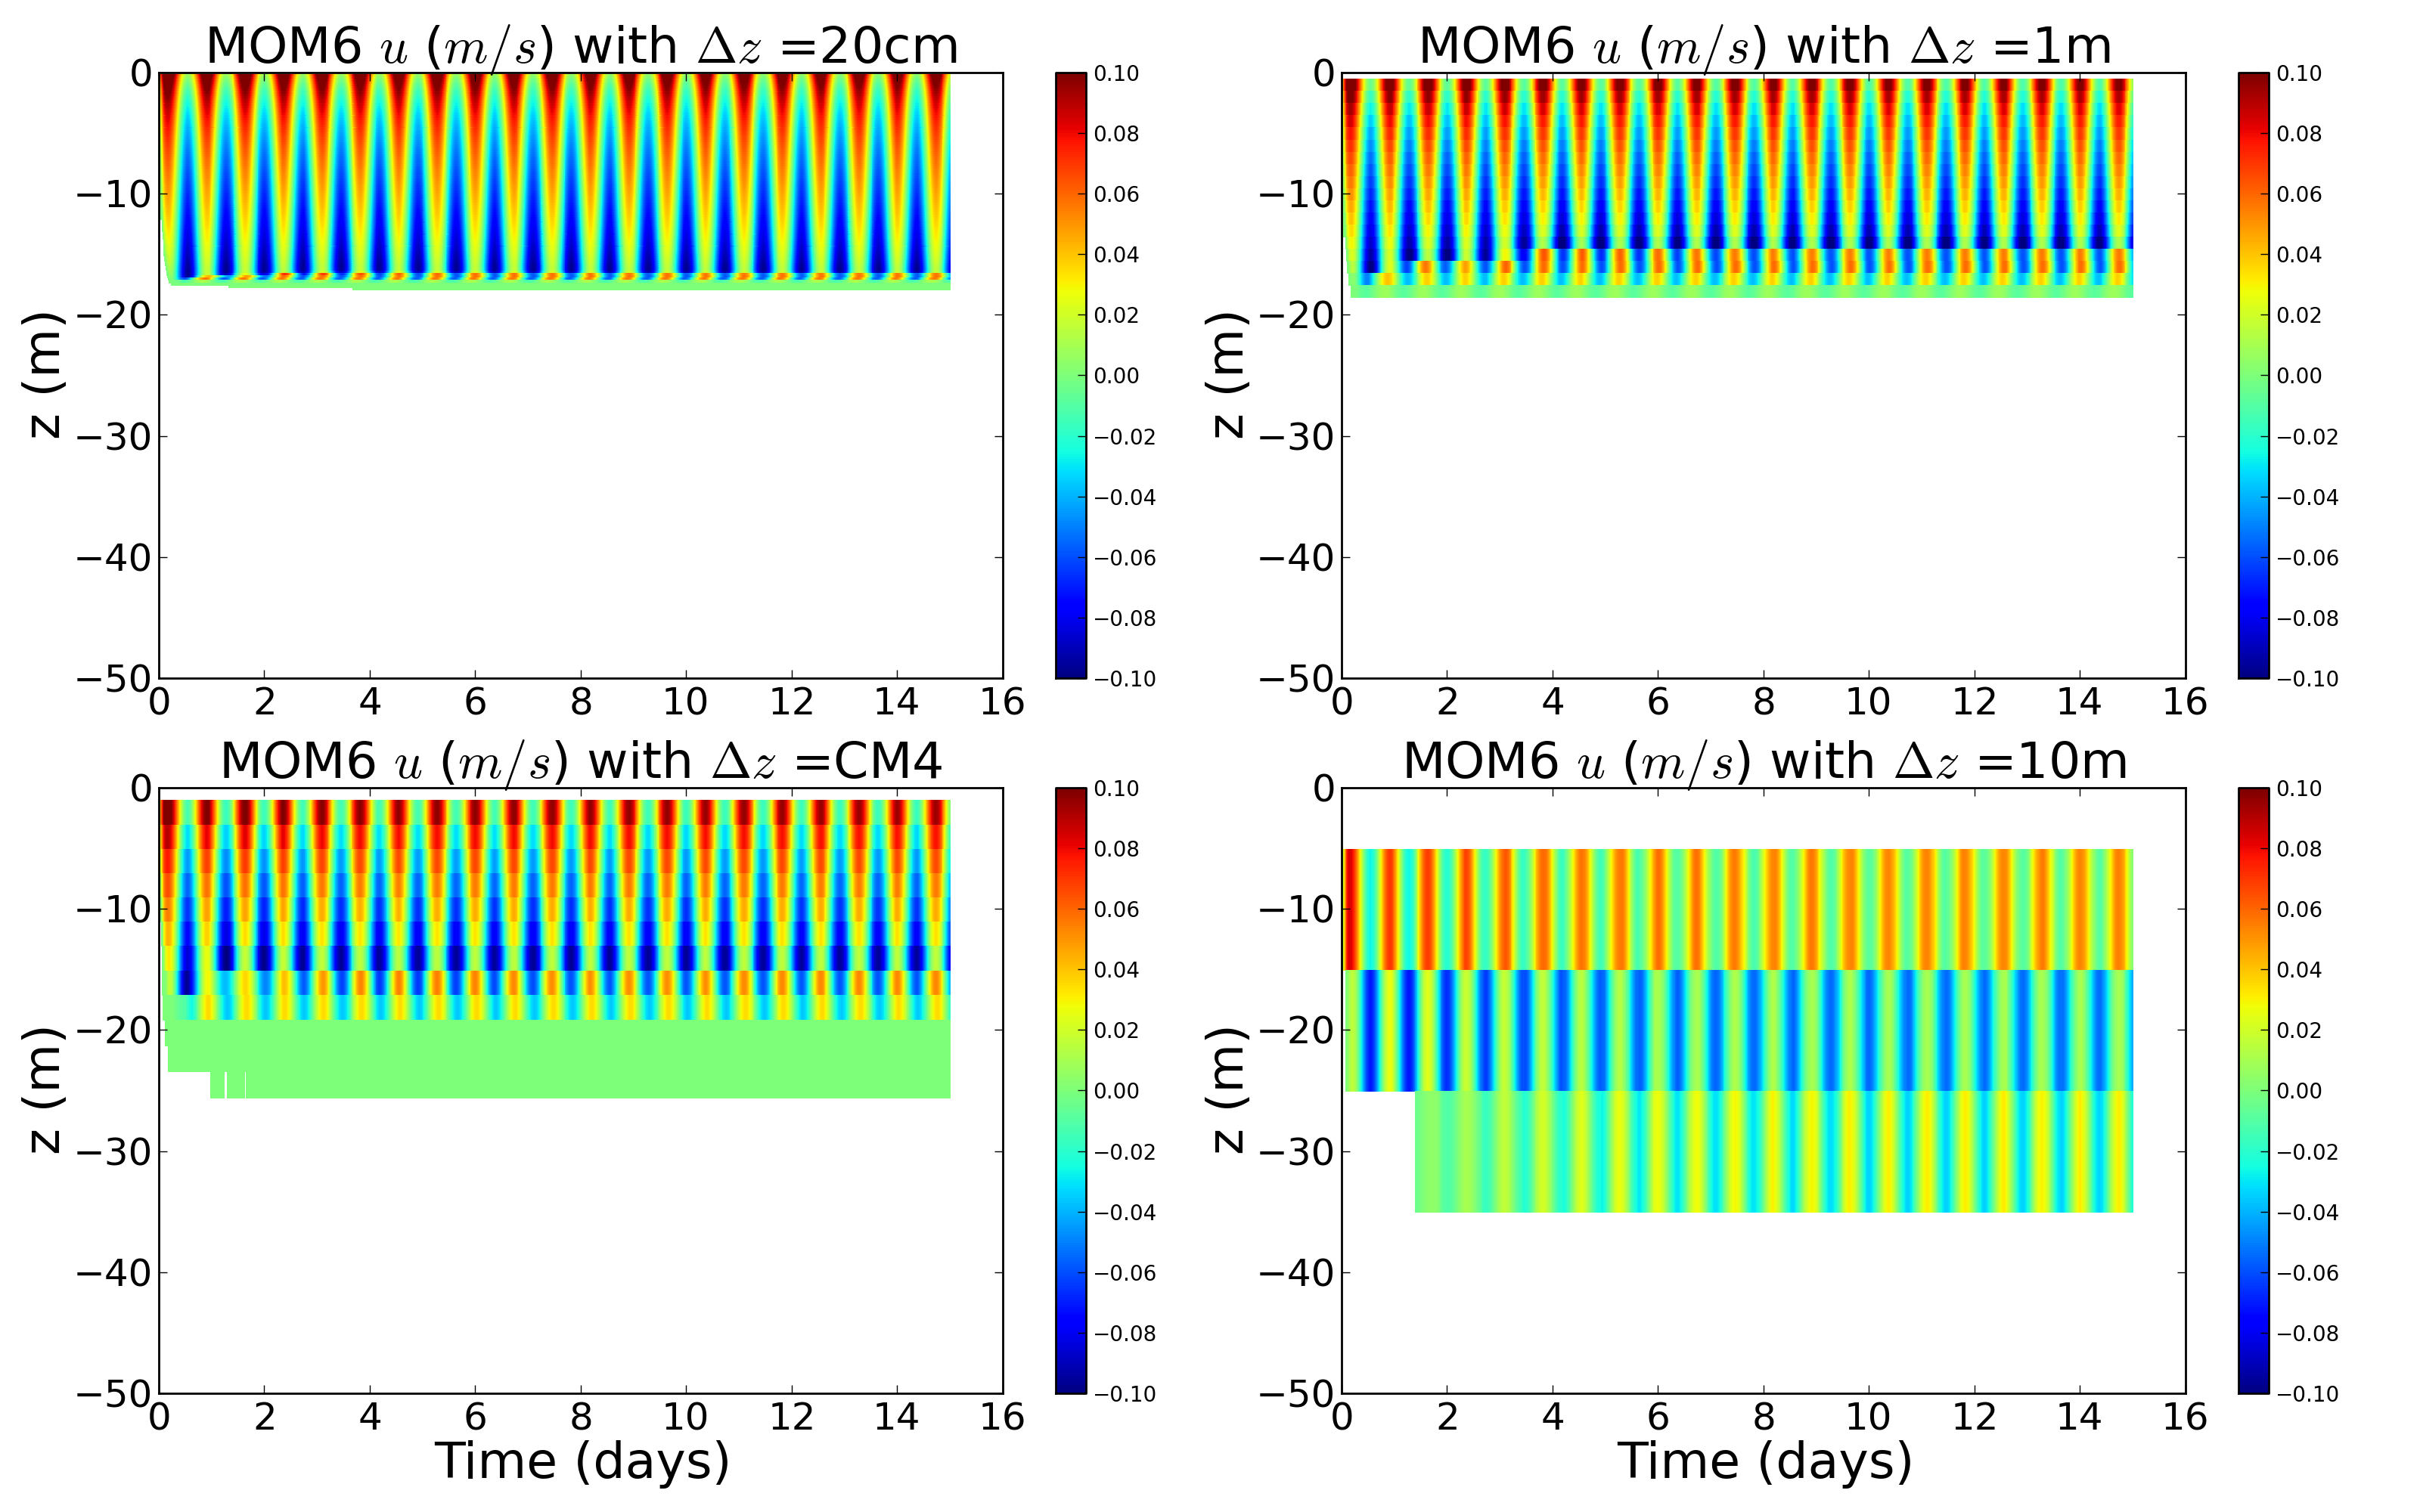
\includegraphics[angle=0,width=14cm]{./figs/MOM6/WSwPSBF_C_MOM6_zonal_velocity.png}
\caption[Zonal velocity from MOM6 for WSwPSBF.C ]{\sf Time series for
  temperature and zonal velocity from test case WSwPSBF.C (constant
  zonal wind stress and restoring heat flux) as realized in MOM6 using
  four different vertical grid resolutions.}
\label{fig:WSwPSBF_C_MOM6_zonal}
\end{center}
%\rule{\textwidth}{0.005in}
\end{figure}
%%%%%%%%%%%%%%%%%%%%%%%%%%%%%%%%%%%%%%%%%%%%%%%%%%%%%%%%%%%%%%%%%%%%%%%%



